%%%%%%%%%%%%%%%%%%%%%%%%%%%%%%%%%%%
%This is the LaTeX ARTICLE template for RSC journals
%Copyright The Royal Society of Chemistry 2016
%%%%%%%%%%%%%%%%%%%%%%%%%%%%%%%%%%%

\documentclass[twoside,twocolumn,9pt]{article}
\usepackage{extsizes}
\usepackage[super,sort&compress,comma]{natbib} 
\usepackage[version=3]{mhchem}
\usepackage[left=1.5cm, right=1.5cm, top=1.785cm, bottom=2.0cm]{geometry}
\usepackage{balance}
\usepackage{mathptmx}
\usepackage{sectsty}
\usepackage{graphicx} 
\usepackage{lastpage}
\usepackage[format=plain,justification=justified,singlelinecheck=false,font={stretch=1.125,small,sf},labelfont=bf,labelsep=space]{caption}
\usepackage{float}
\usepackage{fancyhdr}
\usepackage{fnpos}
\usepackage[english]{babel}
\addto{\captionsenglish}{%
  \renewcommand{\refname}{Notes and references}
}
\usepackage{array}
\usepackage{droidsans}
\usepackage{charter}
\usepackage[T1]{fontenc}
\usepackage[usenames,dvipsnames]{xcolor}
\usepackage{setspace}
\usepackage[compact]{titlesec}
\usepackage{hyperref}
%%%Please don't disable any packages in the preamble, as this may cause the template to display incorrectly.%%%

\usepackage[normalem]{ulem}
\usepackage{xcolor}

\usepackage{epstopdf}%This line makes .eps figures into .pdf - please comment out if not required.

\definecolor{cream}{RGB}{222,217,201}

\begin{document}

\pagestyle{fancy}
\thispagestyle{plain}
\fancypagestyle{plain}{
%%%HEADER%%%
\renewcommand{\headrulewidth}{0pt}
}
%%%END OF HEADER%%%

%%%PAGE SETUP - Please do not change any commands within this section%%%
\makeFNbottom
\makeatletter
\renewcommand\LARGE{\@setfontsize\LARGE{15pt}{17}}
\renewcommand\Large{\@setfontsize\Large{12pt}{14}}
\renewcommand\large{\@setfontsize\large{10pt}{12}}
\renewcommand\footnotesize{\@setfontsize\footnotesize{7pt}{10}}
\makeatother

\renewcommand{\thefootnote}{\fnsymbol{footnote}}
\renewcommand\footnoterule{\vspace*{1pt}% 
\color{cream}\hrule width 3.5in height 0.4pt \color{black}\vspace*{5pt}} 
\setcounter{secnumdepth}{5}

\makeatletter 
\renewcommand\@biblabel[1]{#1}            
\renewcommand\@makefntext[1]% 
{\noindent\makebox[0pt][r]{\@thefnmark\,}#1}
\makeatother 
\renewcommand{\figurename}{\small{Fig.}~}
\sectionfont{\sffamily\Large}
\subsectionfont{\normalsize}
\subsubsectionfont{\bf}
\setstretch{1.125} %In particular, please do not alter this line.
\setlength{\skip\footins}{0.8cm}
\setlength{\footnotesep}{0.25cm}
\setlength{\jot}{10pt}
\titlespacing*{\section}{0pt}{4pt}{4pt}
\titlespacing*{\subsection}{0pt}{15pt}{1pt}
%%%END OF PAGE SETUP%%%

%%%FOOTER%%%
\fancyfoot{}
\fancyfoot[LO,RE]{\vspace{-7.1pt}
\includegraphics[height=9pt]{head_foot/LF}}
\fancyfoot[CO]{\vspace{-7.1pt}\hspace{13.2cm}
\includegraphics{head_foot/RF}}
\fancyfoot[CE]{\vspace{-7.2pt}\hspace{-14.2cm}
\includegraphics{head_foot/RF}}
\fancyfoot[RO]{\footnotesize{\sffamily{1--\pageref{LastPage} ~\textbar  \hspace{2pt}\thepage}}}
\fancyfoot[LE]{\footnotesize{\sffamily{\thepage~\textbar\hspace{3.45cm} 1--\pageref{LastPage}}}}
\fancyhead{}
\renewcommand{\headrulewidth}{0pt} 
\renewcommand{\footrulewidth}{0pt}
\setlength{\arrayrulewidth}{1pt}
\setlength{\columnsep}{6.5mm}
\setlength\bibsep{1pt}
%%%END OF FOOTER%%%

%%%FIGURE SETUP - please do not change any commands within this section%%%
\makeatletter 
\newlength{\figrulesep} 
\setlength{\figrulesep}{0.5\textfloatsep} 

\newcommand{\topfigrule}{\vspace*{-1pt}% 
\noindent{\color{cream}\rule[-\figrulesep]{\columnwidth}{1.5pt}} }

\newcommand{\botfigrule}{\vspace*{-2pt}% 
\noindent{\color{cream}\rule[\figrulesep]{\columnwidth}{1.5pt}} }

\newcommand{\dblfigrule}{\vspace*{-1pt}% 
\noindent{\color{cream}\rule[-\figrulesep]{\textwidth}{1.5pt}} }

\makeatother
%%%END OF FIGURE SETUP%%%

%%%TITLE, AUTHORS AND ABSTRACT%%%
\twocolumn[
  \begin{@twocolumnfalse}
{
\includegraphics[height=30pt]{head_foot/journal_name}\hfill\raisebox{0pt}[0pt][0pt]{
\includegraphics[height=55pt]{head_foot/RSC_LOGO_CMYK}}\\[1ex]

\includegraphics[width=18.5cm]{head_foot/header_bar}}\par
\vspace{1em}
\sffamily
\begin{tabular}{m{4.5cm} p{13.5cm} } 


\includegraphics{head_foot/DOI} & \noindent\LARGE{\textbf{Reassessing structural models of graphitic carbon nitride for reliable photocatalytic predictions$^\dag$}}
\vspace{0.3cm} & \vspace{0.3cm}  \\

 & \noindent\large{Gbemi Abass$^{a\ddag}$, Adnan Ahmad $^{b,c\ddag}$, Cheng Yang $^{b,c}$, Yun Liu $^{b,c*}$, and Terry J.\ Frankcombe$^{a*}$}\\
 
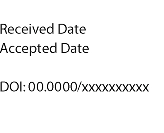
\includegraphics{head_foot/dates} & \noindent\normalsize{Among emerging photocatalysts, graphitic carbon nitride (g-C$_3$N$_4$) has attracted considerable attention as a metal-free, visible-light-active semiconductor for sustainable hydrogen production and environmental remediations.
Here we demonstrate that many of the obvious models for the layer structure and  preferred stacking arrangements of g-C$_3$N$_4$ lead to incorrect predictions of photocatalytic properties. We present a systematic structural exploration of monolayer and bulk geometries of heptazine-based g-C$_3$N$_4$ using first principles density functional theory (DFT) to assess their stability and elucidate how these configurations influence their electronic properties. Across all systems investigated, we show that buckled heptazine structure---rather than the conventional planar geometry---represents the true energetic ground-state structure. Further analysis of buckling and different stacking registries in g-C$_3$N$_4$ layered structures reveals newly identified low-energy corrugated stackings (with $ P1$ symmetry) that give rise to a broad range of electronic band gaps, several of which closely match experimentally reported values of $\sim2.7$ eV. Moreover, introducing non-metal P and metal Ni dopants at identical lattice sites across 2D-planar/buckled and 3D-corrugated hosts shows distinct electronic responses. Our findings demonstrate that accurate structural modelling, including buckling and stacking registry, is crucial for reliably capturing the stability and tunable electronic properties of g-C$_3$N$_4$.  
} 

\end{tabular}

 \end{@twocolumnfalse} \vspace{0.6cm}
 ]
%%%END OF TITLE, AUTHORS AND ABSTRACT%%%

%%%FONT SETUP - please do not change any commands within this section
\renewcommand*\rmdefault{bch}\normalfont\upshape
\rmfamily
\section*{}
\vspace{-1cm}


%%%FOOTNOTES%%%

\footnotetext{\textit{$^{a}$~School of Science, The University of New South Wales, Canberra, ACT 2612, Australia. E-mail: t.frankcombe@unsw.edu.au}}
\footnotetext{\textit{$^{b}$~Research School of Chemistry, The Australian National University, Canberra, ACT 2601, Australia.  E-mail: yun.liu@anu.edu.au}}
\footnotetext{\textit{$^{c}$~ARC Centre of Excellence for Carbon Science and Innovation, Australia}}
\footnotetext{\dag~Supplementary Information available: [details of any supplementary information available should be included here]. See DOI: 00.0000/00000000.}
\footnotetext{\ddag~These authors contributed equally to this work.}


%%%END OF FOOTNOTES%%%


\section{Introduction}
The urgent demand for sustainable energy generation and environmental protection has accelerated interest in solar-driven photocatalysis as a practical route to mitigate these global challenges.\cite{Tong2025RecentPhotocatalysis} Semiconductor-based photocatalysts, capable of harvesting sunlight to drive chemical reactions such as water splitting for hydrogen production, carbon dioxide reduction, and degradation of organic pollutants, provide a clean and scalable approach towards a clean energy future.\cite{Tofil2025ModifiedReview} Among the wide range of semiconductor photocatalysts investigated, graphitic carbon nitride (g-C$_3$N$_4$) has emerged as a promising two-dimensional (2D) metal-free polymeric photocatalyst due to its suitable bandgap for visible light activity, chemical stability, and ease of synthesis, thereby making it highly relevant for various sustainable applications.\cite{Fang2025VersatileApplications,Khan2025RecentReview}

Graphitic carbon nitride exists in two structural frameworks, comprising either s-triazine (C$_3$N$_3$) units or tri-s-triazine (C$_6$N$_7$, also known as heptazine) units. Both structures consist of fused 6-membered rings with sp$^2$ hybridized C and N atoms, forming delocalized $\pi$-conjugated polymeric networks. 
Moreover, as revealed by x-ray diffraction (XRD, Cu target), g-C$_3$N$_4$ is a hexagonal layered structure with two characteristic peaks at approximately 2$\theta$ of 13.04$^\circ$ and 27.6$^\circ$, attributed to the $\langle 10\bar{1}0 \rangle$ in-plane periodicity and $\langle 0002 \rangle$ interlayer stacking governed by weak van der Waals interactions, respectively. While s-triazine and heptazine share a layered graphitic arrangement, heptazine units, consisting of three fused triazine rings, are energetically more favourable.\cite{Zhao2023Two-dimensionalProcesses,PhuongLy2025DecipheringWater,Rizwan2025RoleApplications} Zhang \textit{et al}.\cite{Zhang2025FunctionalNitride} report the structural evolution from triazine to heptazine during thermal polymerization and highlights new theoretical insights for synthesizing heptazine-based g-C$_3$N$_4$ at lower temperatures.

Unlike graphene, which consists mainly of carbon atoms, polymeric g-C$_3$N$_4$ contains both carbon and nitrogen atoms, resulting in increased structural complexity. Consequently, uncertainty regarding the precise structure of polymeric g-C$_3$N$_4$ and the identification of its true ground-state structure continues to present significant challenges for both experimental and theoretical investigations. For example, the conventional synthesis route of polymeric carbon nitride, such as thermal polycondensation in air, typically yields a semicrystalline structure with mixed motifs, thereby complicating precise structural characterization.\cite{Negro2023CombinedProperties}
The reduced crystallinity of g-C$_3$N$_4$ is commonly attributed to incomplete polymerization and the persistence of hydrogen bonding within the synthesized sample, which results in a partially condensed framework of a melon-type g-C$_3$N$_4$ structure.\cite{Im2023StructureSimulations}

Recently, Negro \textit{et al}.\cite{Negro2023CombinedProperties} conducted a combined experimental and theoretical investigation on g-C$_3$N$_4$ structure using different characterization techniques such as XRD, FTIR, SEM, UV-Vis, and data from density functional theory tools. Their study demonstrated that thermal polymerization of melamine produces a mixture of structural motifs comprising less-condensed melon frameworks together with highly condensed g-C$_3$N$_4$ domains. Another study by Zhang \textit{et al}.\cite{Zhang2023Salt-MediatedPhotocatalysis} provides insights into the structural transformation mechanism of g-C$_3$N$_4$ synthesized via a molten salt-assisted procedure. They report a sequential phase evolution in which melon converts first into poly(heptazine imide) as an intermediate phase, and subsequently into poly(triazine imide) as the more stable phase. Collectively, earlier works have demonstrated that the structure, and consequently the properties, of g-C$_3$N$_4$ can be modulated via different synthesis routes such as precursor composition, condensation temperature, reaction rates and related factors.\cite{Ma2024TheModification,Zhang2025FunctionalNitride} Nonetheless, the fundamental question of what is the ground state structure of fully polymerized heptazine-based g-C$_3$N$_4$ has not been answered through experimental investigation. 

In an effort to resolve the true ground state of pure heptazine-based  g-C$_3$N$_4$, numerous theoretical investigations based on first-principles density functional theory (DFT) and molecular dynamics have been conducted.\cite{Wang2018TheStudy,Wang2017DeterminationValidation,Gao2020CorrugationStudies}
While numerous studies employ a graphene-like planar model of $P\bar{6}m2$ symmetry for the g-C$_3$N$_4$ layer structure, other studies have allowed the geometry to flex into nonplanar structures.
Recent theoretical work\cite{Im2023StructureSimulations,Fao2022TheoreticalPd,Hartley2021ComputationalSplitting} has demonstrated that out-of-plane structures, such as buckled or corrugated layers, are energetically more favourable and offer a more realistic model of the fully polymerized heptazine phase. Moreover, Zhao \textit{et al}. \cite{zhao2021NewNitride} proposed three corrugated structures of $P321$, $P3m1$ and $Pca2_1$ symmetry for experimentally sythesized g-C$_3$N$_4$. These were found to be energicatlly more stable than the conventional flat $P\bar{6}m2$ model. Other theoretical investigations  that adopted a flat g-C$_3$N$_4$ model as the initial structure for adsorption or dopant studies consistently yielded buckled configurations, with planarity not being preserved once the symmetry is broken in the calculation.\cite{Azofra2016AConversion,Zhou2022TheStudy,Zhang2017PhotocatalyticG-C3N4b,Ji2016Heptazine-basedMembrane} These observations collectively suggest that out-of-plane buckling is an intrinsic feature of g-C$_3$N$_4$. However, it remains challenging, experimentally, to detect the subtly buckled heptazine phase.
When the basal plane of the layered structure is viewed from above
(with atomic-resolution microscopy techniques) the corrugated and planar g-C$_3$N$_4$ structures would be virtually indistinguishable.

Another important consideration in the search for the true ground state of heptazine-based g-C$_3$N$_4$  requires careful evaluation of how the two-dimensional (2D) layers are arranged to form a stacked three-dimensional (3D) bulk structure. The different stacking configurations between adjacent g-C$_3$N$_4$ sheets play a decisive role in determining the structural stability and electronic properties of the bulk phase. Although many theoretical studies\cite{Yang2021DFTApplications,Fu2024PotassiumInvestigation,Gorai2023InsightPrinciple} have modelled exfoliated  g-C$_3$N$_4$ as an isolated monolayer to rationalize enhanced photocatalytic activity, the persistence of the (0002) diffraction peak indicates evidence of residual interlayer stacking. As a result, interlayer interactions and $\pi$-$\pi$ overlap between adjacent sheets must not be neglected in describing the ideal phase of heptazine-based g-C$_3$N$_4$. In 2018, Sun \textit{et al.} \cite{Sun2018FirstArrangement} investigated the electronic properties of graphitic carbon nitride with different building blocks and staggered between sheets in the bulk phase. In their study, triazine- and heptazine-based structures were examined under different stacking configurations ($P\bar{6}m2$, $R3m$, $Cmcm$, and $P6_3/mmc$), and the results showed that bulk g-C$_3$N$_4$ polymorphs exhibit narrower band gaps than the corresponding monolayers, with the reduction attributed to interlayer band overlap between adjacent CN sheets. Other previous studies 
have also indicated that polymeric carbon nitride comprises stacked layers that preferentially adopt AB stacking registries as compared 
to AA.\cite{Hartley2021ComputationalSplitting,Zuluaga2015StructuralG-C3N4}
However, the precise stacking order and local structural motifs remain uncertain due to experimental constraints, motivating further investigation. 

A more recent study \cite{Im2025UnravelingTransitions} demonstrated that the electronic and optical responses of polymeric g-C$_3$N$_4$ are dependent on the microstructural features, particularly the degree of condensation, out-of-plane corrugation, and interlayer interactions. These conclusions are consistent with prior work,\cite{Im2023StructureSimulations,Negro2023CombinedProperties} providing a strong rationale to systematically investigate the effect of buckling and stacking configurations in developing a more robust theoretical model for the fully condensed heptazine phase of g-C$_3$N$_4$.

Mridha \textit{et al}. \cite{Mridha2025UsingG-C3N4} recently advanced the earlier work of Im and colleagues \cite{Im2025UnravelingTransitions} by providing a dynamic analysis of the ground-state structure of g-C$_3$N$_4$, systematically examining heptazine-, h-triazine-, and o-triazine-based polymorphs in both bulk and monolayer models. Their phonon calculations revealed that all planar polymorphs are dynamically unstable and relax to buckled structures, with heptazine identified as the energetically preferred structure. 

While earlier studies have confirmed that buckling is intrinsic to the stability of g-C$_3$N$_4$, their scope remained limited to idealized monolayers and bulk phases, without assessing the influence of stacking registries on the relative stability of corrugated heptazine structures. To address this gap, the present study systematically investigates the interplay between buckling and different stacking configurations in heptazine-based g-C$_3$N$_4$, with a direct comparison between planar/buckled monolayers and the energetically preferred corrugated bulk phase. In addition, we have investigated how altering the assumed buckling and stacking structure affects the properties of phosphorus and nickel doping of g-C$_3$N$_4$. Our results reveal that the combination of buckling and appropriate stacking configurations stabilizes heptazine by yielding lower-energy corrugated structures.





\section{Computational Details}
All periodic first-principles calculations performed in this study were carried out using the plane-wave density functional theory (DFT) as implemented in the Vienna Ab-initio Simulation Package (VASP) code.\cite{Kresse1996EfficiencySet},\cite{Kresse1999FromMethod} The interaction between ionic cores and valence electrons was described using the projector-augmented-wave (PAW) potentials provided with VASP. 

\begin{figure*}
  \centering
  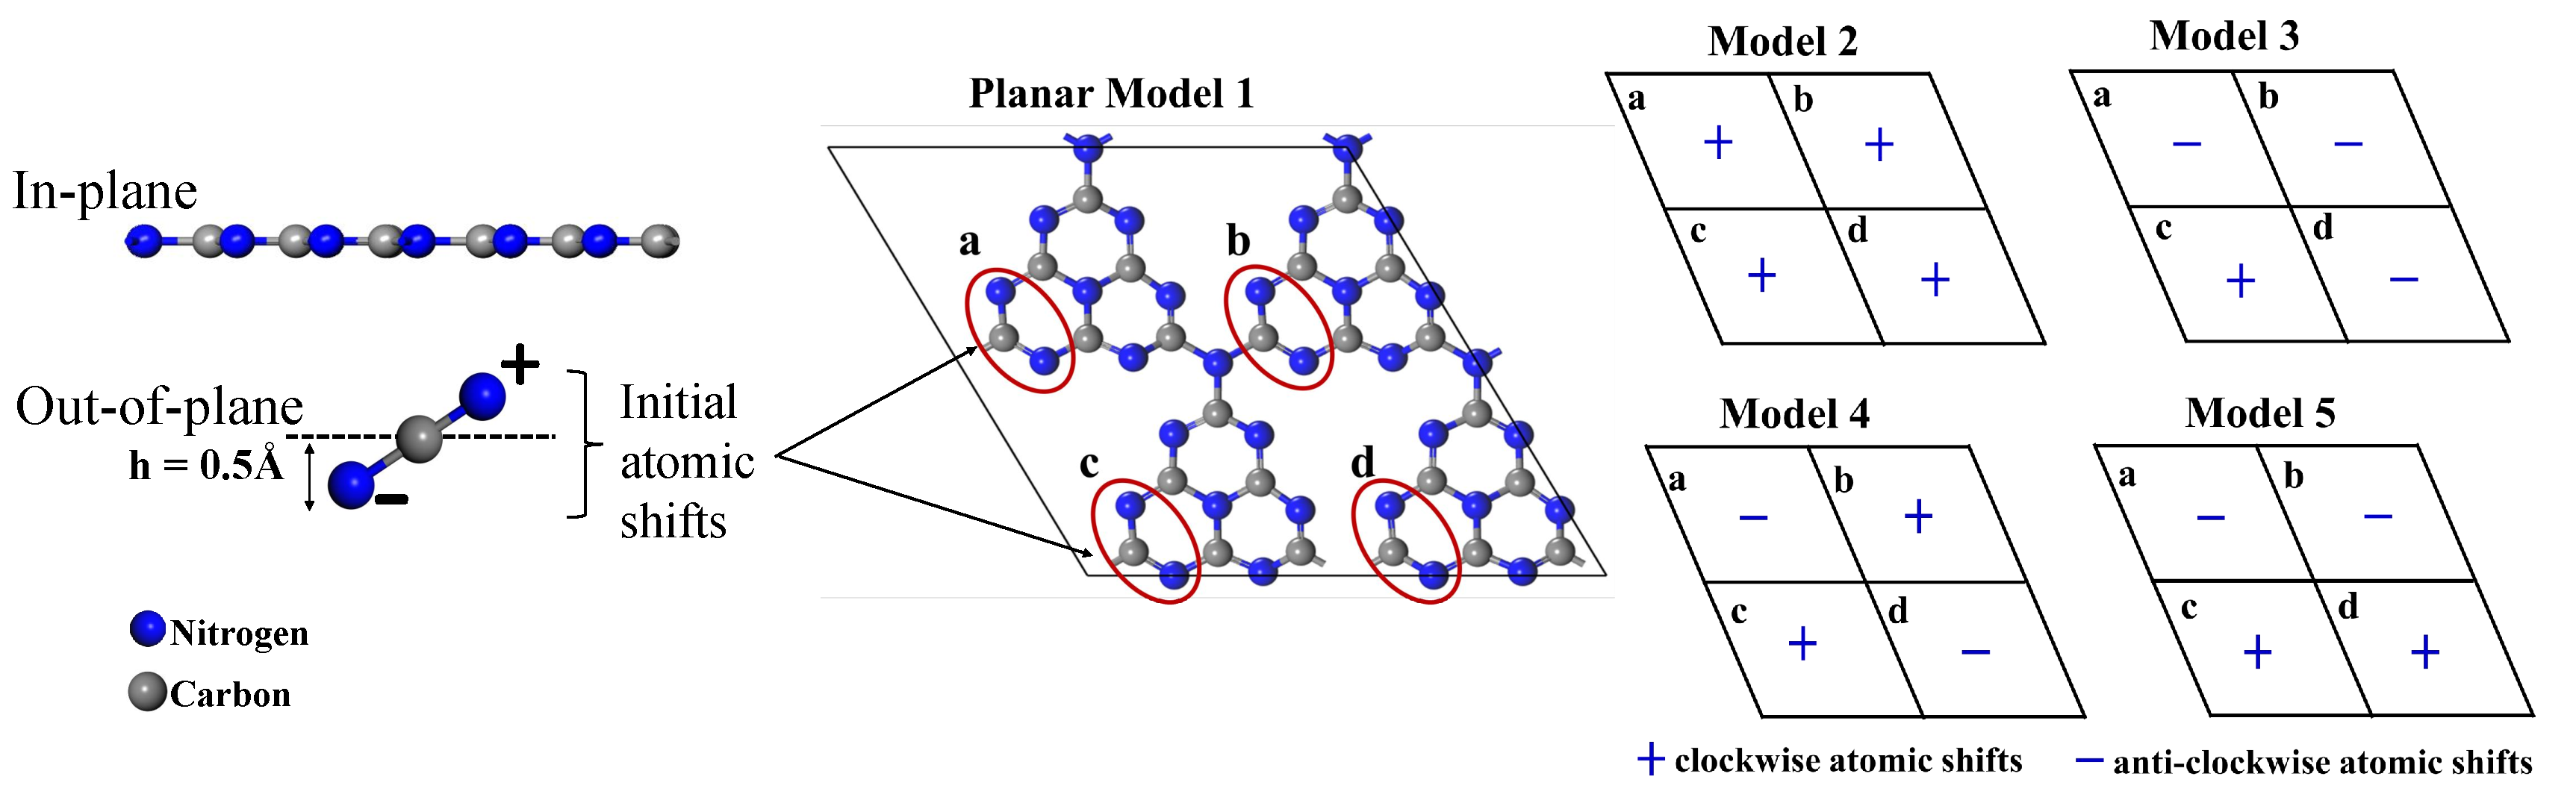
\includegraphics[width=6.5in]{Figures/Fig1.pdf}
 \caption{Exploration of low-energy g-C$_3$N$_4$ buckling patterns initiated by atomic shifts/distortions of the planar monolayer.} 
  \label{fig:Fig1} 
\end{figure*}

Exchange-correlation energies were treated within the generalized gradient approximation (GGA) using the Perdew-Burke-Ernzerhof (PBE) functional. To properly account for weak interlayer interactions in the bulk models, van der Waals corrections were included using the DFT-D3 scheme\cite{Grimme2010AH-Pu} with Becke-Johnson damping. The PBE functional without dispersion corrections as well as the r$^2$SCAN meta-GGA and HSE06 screened hybrid functionals were used for specific comparisons, as noted in the results presented below. These functionals were applied at the geometries that minimize the PBE-D3(BJ) energy. To assess the robustness of the predicted structure, one representative bulk structure was also fully optimized using different functionals (see Table S3 and Fig. S3). The plane wave energy cutoff was set as 500 eV, while the self-consistency energy convergence criterion was set to 10$^{-6}$ eV. 
All structures were based on layers comprised of $2 \times 2$ supercells of the heptazine monomeric unit and an accompanying pore. The Brillouin zone was sampled using $\Gamma$-centered k-point meshes, specifically a $3 \times 3 \times 1$ grid for 2D structures (incorporating a nominally 20~\AA\ gap between layers) and a $3 \times 3 \times 7$ grid for the 3D bulk systems. These grid point meshes were selected based on convergence tests that confirmed they are well-converged with respect to total energy (see Fig. S1). 

To systematically search for lower-energy configurations, we introduced out-of-plane shifts of 0.5~\AA\ for different atoms within heptazine to break the planar symmetry as depicted in Fig.\ \ref{fig:Fig1}. The monolayer was partitioned into four symmetry-related regions labelled a, b, c, and d. Each label corresponds to two pyridinic nitrogen atoms (N$_2$C sites), which are two-coordinated nitrogen atoms bonded to two carbon atoms within each heptazine unit. These N$_2$C atoms serve as the primary sites where out-of-plane perturbations were applied to initiate buckling. Model 1 represents the planar reference structure without any atomic perturbation, whereas Models 2 to 5 incorporate systematic clockwise ($+$) and anti-clockwise ($-$) out-of-plane atomic shifts. 

To determine the stability of P and Ni dopants in the 2D/3D g-C$_3$N$_4$ structures, we carried out spin-polarized DFT calculations.  The energy required to create a substitutional defect ($E_{\text{form}}^{\text{sub}}$) and an interstitial defect ($E_{\text{form}}^{\text{int}}$) were calculated using the following formation energy equations:
\begin{equation}
E_{\text{form}}^{\text{sub}} = E_{\text{doped}} - E_{\text{undoped}} - \mu_{\mathrm{dopant}} + \mu_{\mathrm{C/N}}
\label{eq:formation_energy_sub}
\end{equation}
\begin{equation}
E_{\text{form}}^{\text{int}} = E_{\text{doped}} - E_{\text{undoped}} - \mu_{\mathrm{dopant}}
\label{eq:formation_energy_int}
\end{equation}
where $E_{\text{doped}}$ and $E_{\text{undoped}}$ are the total energies of the doped and pristine supercells, $\mu_{\mathrm{dopant}}$ is the chemical potential of the added dopant atom, while $\mu_{\mathrm{C/N}}$ corresponds to the chemical potential of the atom that occupied the substitution site prior to doping (either C or N).
The chemical potential terms were taken as the per atom energy from the relevant pure phase: black phosphorous for P, metallic nickel for Ni, graphite for C and molecular dinitrogen (isolated in a large periodic box) for N.  Care was taken to converge the k-point grids for these pure phase calculations (Fig.~S7) to ensure that the corresponding uncertainties in Eqs.\ (\ref{eq:formation_energy_sub}) and (\ref{eq:formation_energy_int}) due to sampling were significantly smaller than the values quoted in this work.
A single dopant atom was used in each $2 \times 2$ supercell for the single layer stuctures and one dopant atom in the two layer supercell for the bulk structures.

The interlayer binding energy was calculated using the expression:\cite{Bian2022StrongMaterials,Jung2018APrinciples}
\begin{equation}
E_b = \frac{2E_{\rm single-layer} - E_{\rm bulk}}{2A}
\label{eq:binding}
\end{equation}
where \(A\) is the basal-plane area of the bulk unit cell, \(E_{\rm single-layer}\) is the total energy of the optimized monolayer, and \(E_{\rm bulk}\) is the total energy of the corresponding two-layer bulk supercell.

A limited investigation of molecular heptazine dimers was conducted using the Gaussian 16 code.\cite{Frisch2016GaussianC.01}  
Two heptazine molecules (C$_6$N$_7$H$_3$) were brought together edge to edge in a constrained relaxation, controlling the N-N distance of one intermolecular pair and maintaining the planes of the two molecules at right angles to isolate the N-N lone pair interaction. The MP2/def2-SVP level of theory was used for dimer calculations.
Moreover, limited Reverse Monte Carlo (RMC) simulations were performed on X-ray total scattering data from synthesised samples of g-C$_3$N$_4$.\cite{Adnan2026atomicallycoordinatednonmetal}  These simulations were performed with the RMCProfile code.\cite{Tucker2007RMCProfile:Materials,Liu2025HarnessingCapacitors,Wang2025RegulatedFixation}
Starting from a 10000 atom supercell of planar bulk g-C$_3$N$_4$, the RMC iteratively perturbs the positions of these atoms until the calculated scattering pattern matches the experimentally measured data.

\section{Results and Discussion}
\subsection{Structural stability of g-C$_3$N$_4$ monolayer}
We begin our discussion with the $2 \times 2$ supercell of the flat heptazine monolayer, constructed from its unit cell ($a=b=7.1~\text{\AA}$). Upon geometry relaxation using the PBE functional, the planar configuration persisted as an in-plane heptazine network with supercell lattice constants of $a = b = 14.2$~\text{\AA} (Fig.\ \ref{fig:Fig2}a), consistent with previous theoretical work.\cite{Gao2017TheStudy,Wu2014TheNitride}
However, the optimized flat model is an unstable stationary point.
Displacements in the positive and negative $z$ directions are symmetry equivalent so that the $z$ components of calculated forces remain exactly zero even though 
out-of-plane distortion lowers the energy.
A series of controlled out-of-plane perturbations was therefore introduced to the planar geometry as shown in Fig.\ \ref{fig:Fig1} to systematically search for lower-energy configurations. Each of these perturbed structures was subsequently relaxed to yield buckled configurations lower in energy than the planar reference (Model 1), as summarized in Table S1. 
Among the corrugated structures considered, Model 4 (defined by alternating clockwise and anti-clockwise atomic shifts in the pattern indicated in Fig.\ \ref{fig:Fig1}) emerged as the most stable, with the supercell about 2.9 eV lower in energy than the flat configuration at the PBE level. This energetic preference was consistent across other tested exchange-correlation functionals (r$^2$SCAN and HSE06), providing strong evidence that the corrugated model offers the most realistic description of the ground state of single-layer heptazine-based g-C$_3$N$_4$. As shown in Fig.\ \ref{fig:Fig2}b, the optimized buckled configuration (Model 4)
was adopted as the representative corrugated model for heptazine monolayer in our study. As compared to the planar sheet (Fig.\ \ref{fig:Fig2}a), the buckled structure relaxed to a reduced lattice constant of 13.9~\text{\AA} with a buckling height of 1.35~\text{\AA}, consistent with other studies.\cite{Gao2020CorrugationStudies,Mridha2025UsingG-C3N4, Liu2020StructuralInvestigation}. 
Analysis of the structure after relaxation revealed that the planar model retained elongated bridge N-C bonds ($\sim1.47$~\text{\AA}), whereas the buckled structure allowed these bonds to contract slightly to $\sim1.42$~\text{\AA}.
The remaining N-C bonds increased slightly from 1.33 to $\sim1.35$~\text{\AA}, reflecting redistribution of local strain. 

\begin{figure*}
  \centering
  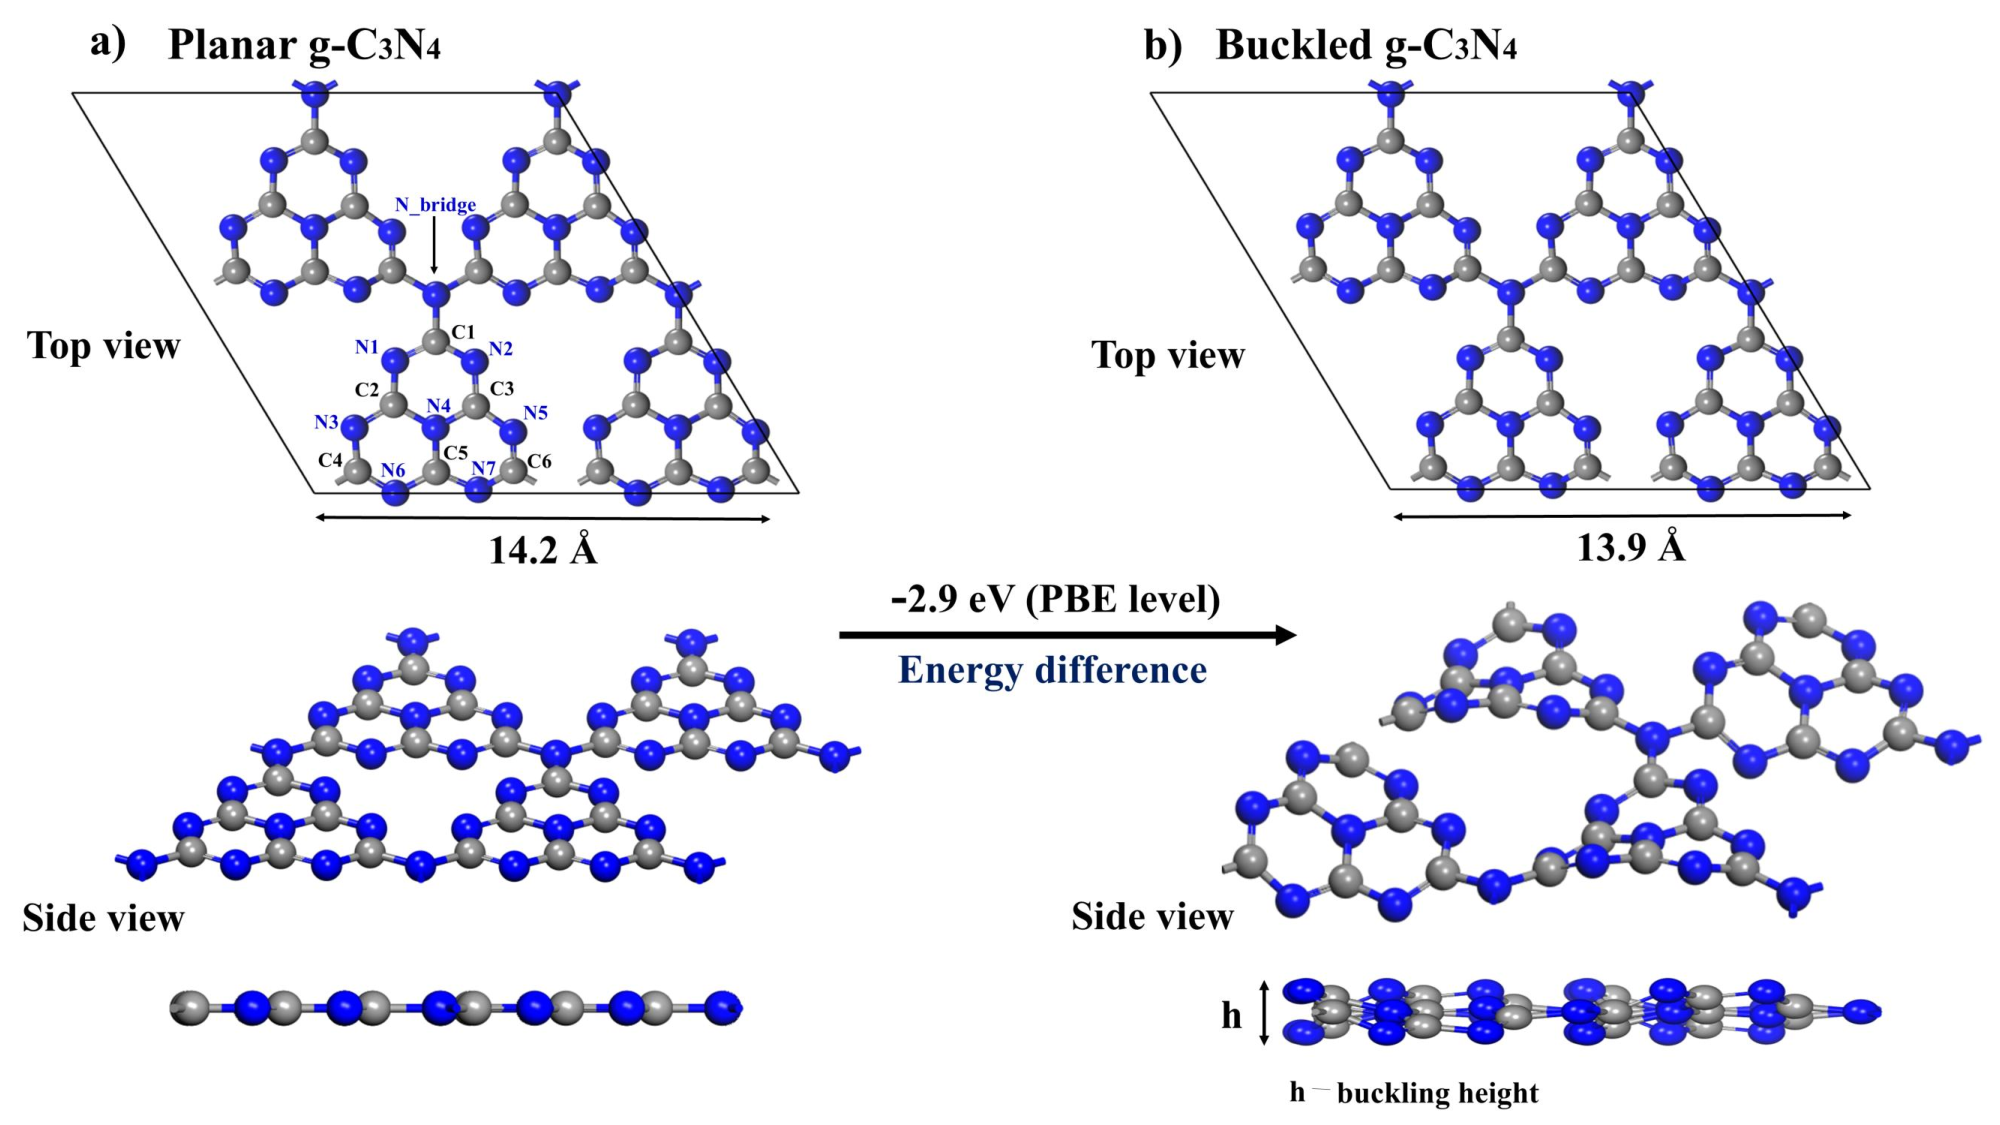
\includegraphics[width=5.6in]{Figures/Fig2.pdf}
 \caption{Relaxed 2x2 supercell of (a) planar and (b) buckled heptazine-based g-C$_3$N$_4$ monolayers.} 
  \label{fig:Fig2} 
\end{figure*}

Note that the energy difference between our Model 4 and the flat Model 1 is significantly larger than the differences found by Mridha \textit{et al.}\cite{,Mridha2025UsingG-C3N4}
The periodicity of the single heptazine cell used by this earlier work limits
the structures that can be found by their phonon-following approach to be of our Model 2 type (c.f.\ Fig.\ \ref{fig:Fig1}).

The shortening of the bridging C-N bonds upon buckling suggests buckling relieves steric hinderance between lone pairs of non-bonded nitrogens on the heptazine edges.  This was investigated briefly by examining the 
potential energy profile of two heptazine molecules (C$_6$N$_7$H$_3$) brought together edge to edge in a constrained relaxation, controlling the nearest intermolecular N-N distance.
Increasing the N-N distance from the 2.4~\AA\ found in the flat structure to the 2.7~\AA\ of the buckled geometry decreased the total energy by 0.43~eV at the MP2/def2-SVP level.  As there are twelve such ``intermolecular'' N-N pairs in heptazine g-C$_3$N$_4$, this represents a significant reduction in energy through relief of these clashing electron-rich atoms.  
Although there will be some contribution from different levels of theory [MP2 versus DFT with PBE-D3(BJ)], that the total reduction of energy upon buckling is significantly less than $12\times 0.43$~eV suggests that strain within the structure on buckling limits the distortion.

Our Model 4 structure exhibits antiphase distortions 
(i.e.\ alternating distortion directions) along the $\langle 10\bar{1}0\rangle$
and $\langle 01\bar{1}0\rangle$ directions.  This suggests energetic coupling 
between distortions similar to antiferroelectric coupling in ionic crystals.
Such an interpretation would make the distortions frustrated on the hexagonal 
lattice of g-C$_3$N$_4$, as the symmetry-equivalent $\langle \bar{1}100\rangle$ direction cannot simultaneously exhibit antiphase ordering in this finite
$2 \times 2$ instantiation of the structure.  Thus one may expect significant 
dynamical fluctuations of the out-of-plane distortion structure in real g-C$_3$N$_4$ crystals.

Our findings further support earlier reports\cite{zhao2021NewNitrideb,Mortazavi2025AMonolayers} that corrugated structures resemble the flat g-C$_3$N$_4$ model (Fig.\ \ref{fig:Fig2}) when viewed from above the basal plane, which led to the widely used flat (metastable) $P\bar{6}m2$ model in previous theoretical studies to interpret experimental data. However, having established the buckled configuration as the true energy minimum for the single-layer heptazine model, we proceed to examine the interlayer interactions and stacking registries of these corrugated sheets. The motivation to extend this structural investigation arises from experimental observations showing that exfoliated g-C$_3$N$_4$ nanosheets often retain interlayer spacings corresponding to the (0002) reflection in X-ray diffraction patterns. Moreover, while the precise interlayer registry of heptazine-based g-C$_3$N$_4$ remains unresolved, the stacking configuration cannot be neglected when accurately describing the synthesized heptazine sample. Therefore, in the following section, we systematically explore different stacking possibilities of heptazine-based g-C$_3$N$_4$ using first-principles theoretical calculations.

\subsection{Stacking motifs in bulk g-C$_3$N$_4$}
Similar to graphite, g-C$_3$N$_4$ consists of 2-dimensional layers held together by weak van der Waals forces, allowing adjacent sheets to take on a range of lateral displacements and orientations.
This results in different stacking configurations, which constitute a fundamental structural variable that can be exploited to modulate the electronic and optical properties of g-C$_3$N$_4$.\cite{Bao2017Stacking-DependentSpectroscopy,Fox2024StackingApplications}
We systematically investigated different stacking configurations of layered heptazine-based g-C$_3$N$_4$.

\begin{figure*}[h!]
  \centering
  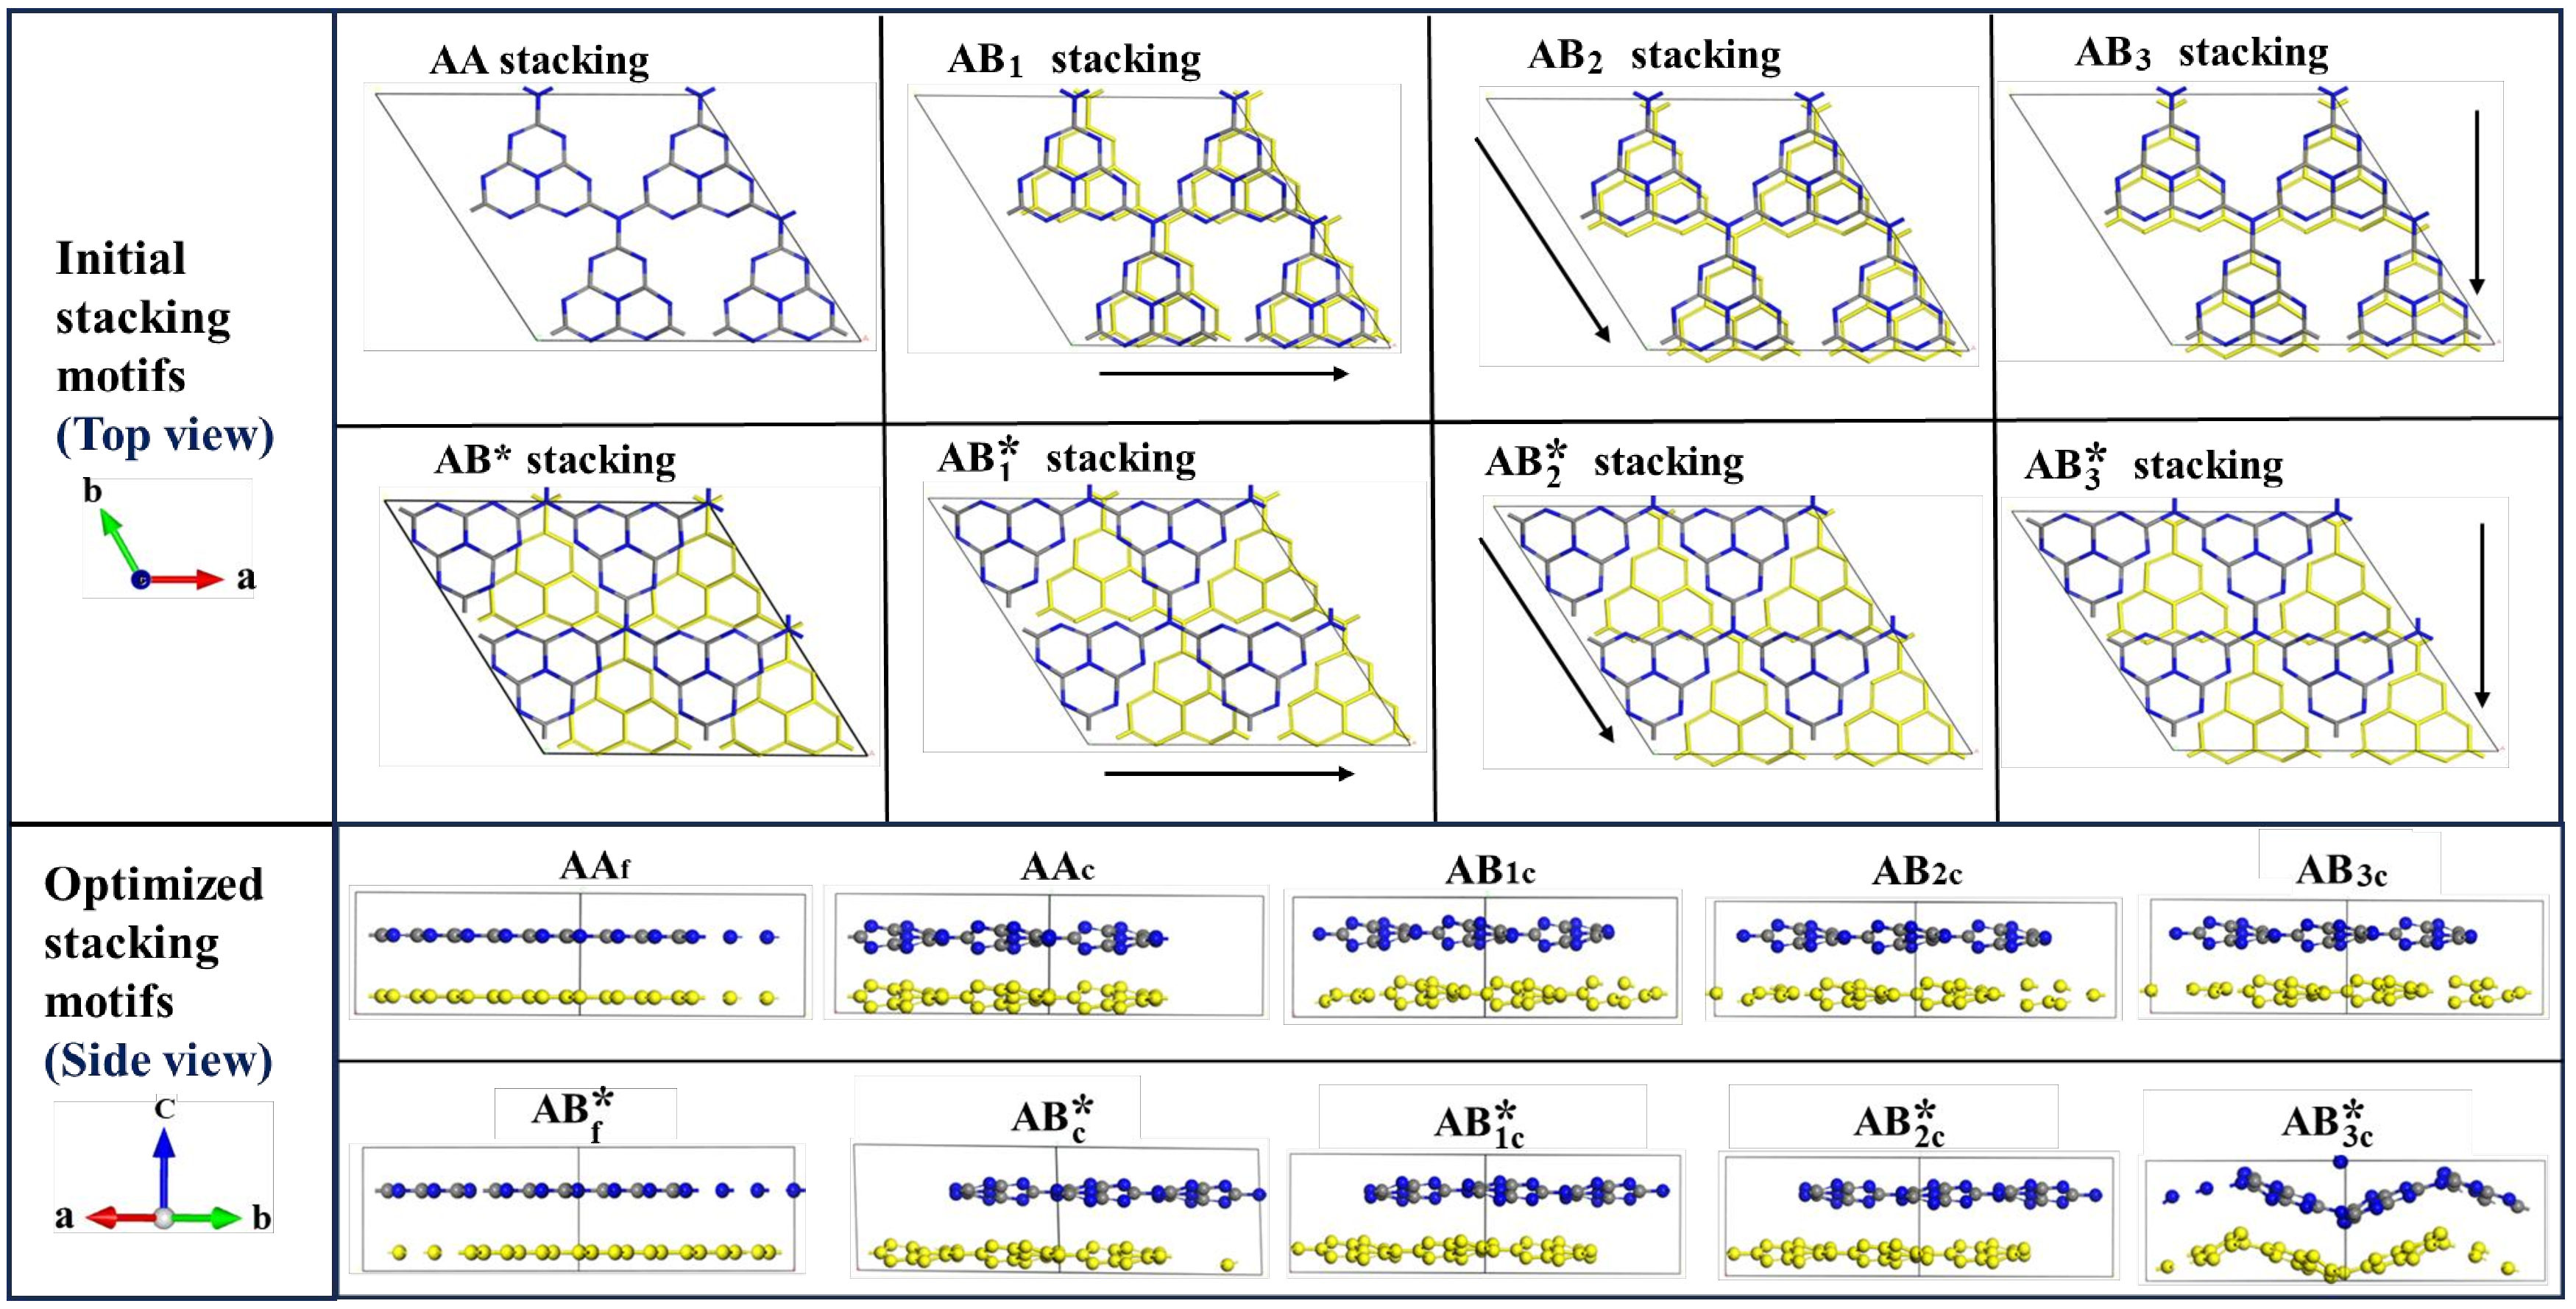
\includegraphics[width=6.8in]{Figures/Fig3.pdf}
 \caption{Structural investigation of different stacking motifs of heptazine-based g-C$_3$N$_4$ in both flat and buckled models to identify the most stable configuration. The asterisk (*) and subscripts c and f refer to 180$^\circ$ rotation, corrugated, and flat models, respectively. 
 The side views are along the $[11\bar{2}0]$ direction.} 
  \label{fig:Fig3} 
\end{figure*}

A series of initial configurations was tested to search for the most favourable
interlayer configurations.  In all cases we use a supercell comprising two layers of g-C$_3$N$_4$ sheets, yielding $2 \times 2$ supercells of the heptazine monomer.  These are illustrated in Fig.\ \ref{fig:Fig3}.

The bulk material with no lateral shift between each layer is denoted AA stacking.
A range of AB-type stacking patterns were generated for testing. Those we label AB$_{1}$, AB$_{2}$ and AB$_{3}$ were generated by introducing an initial lateral shift of 0.6~\text{\AA} along the $\mathbf{a}$, $-\mathbf{b}$ or $-2\mathbf{b}-\mathbf{a}$
directions, respectively, from the AA structure for every other layer.
Another set of 180$^\circ$-rotated AB variants was modelled, in which one flat or corrugated layer was first rotated by 180$^\circ$ relative to the perfectly aligned AA stacking. In this arrangement, the carbon atoms lie within the void regions, while only some nitrogen atoms, including the bridging nitrogen atoms (not carbon), overlap. As seen in Fig. \ref{fig:Fig3}, AB* is used to denote the structure resulting solely from this rotation, a structure that is usually denoted simply AB in other work.
We also consider applying similar lateral shifts to those described above from this AB* structure, denoted AB*$_{1}$, AB*$_{2}$ and AB*$_{3}$. This notation was extended with an additional 
subscript $f$ or $c$ to distinguish between structures constructed from flat or corrugated g-C$_3$N$_4$ layers, respectively. For example, AB*$_{2c}$ is a staggered model comprising corrugated layers of alternating orientation that has been initially shifted along the $\mathbf{b}$ axis.%
\footnote{Note that, at the time of writing, the structure labelled here as $AB^*_f$ is listed as the stable structure in the Materials Project online database.}
All structures were relaxed with the PBE-D3(BJ) functional.

The optimized lattice parameters, lattice angles, and relative energies [computed using various exchange-correlation (XC) functionals] for each configuration are presented in Table \ref{tab:stacking}. 
Consistent with previous theoretical studies, \cite{Sun2018FirstArrangement,Zuluaga2015StructuralG-C3N4}
the flat AA$_f$ reference model (with lattice constants $a = 14.2$~\text{\AA} and $c = 6.73$~\text{\AA}) was the highest energy structure. 
However, introducing a 180$^\circ$ rotation in the flat AB$_f$ stacking motif, denoted as AB*$_f$, lowers the energy by $\sim3.1-4.0$ eV across all the XC functionals, highlighting that changes in the stacking registry can significantly influence structural stability. In contrast, the corrugated AA$_c$ structure undergoes an in-plane contraction ($a = 6.95$~\text{\AA}) and a slight expansion along $c$ ($\sim7.18$ ~\text{\AA}) and lowers the energy by $\sim6.6$ eV. The enhanced stability of the AA$_c$ stacking configuration, relative to the previously discussed models, can be attributed to the relief of interlayer electrostatic repulsion through out-of-plane buckling.

Modifying the interlayer arrangement in the corrugated bulk structure results in a further reduction in total energy, with the AB$_3c$ registry attaining the lowest relative energy (-7.81 eV at the HSE level) within this stacking series. Moreover, among the 180$^\circ$-rotated corrugated stacking series, AB*$_c$ shows moderate stability, whereas the addition of translational shifts in AB*$_3c$ motif achieves the lowest energy stacking configuration across all the XC functionals. Consistent with these structural relaxations, the corrugated stacking registries exhibit buckling heights ranging from $\sim 0.97$ to $2.84$~\AA, including $1.28$~\AA\ for AAc and $0.97$~\AA\ for AB$^{*}_{c}$, while the AB$_{1c}$--AB$_{3c}$ motifs show distortions of $\sim 1.31$--$1.42$~\AA, reaching up to $2.84$~\AA\ for AB$^{*}_{3c}$.

To further investigate the interlayer coupling strength of the various stacking registries in g-C$_3$N$_4$ the interlayer binding energy is considered. This provides a quantitative measure of the cohesion between adjacent heptazine sheets. 

The interlayer binding energy is calculated using Eq.\ (\ref{eq:binding}). 
Table S2 provides details of the interlayer binding energies for all planar and corrugated stacking registries. Across these configurations, the binding energy values fall within 6--17~meV\,\AA$^{-2}$, lower than the binding/exfoliation energies of some other van der Waals materials such as graphene (22.5~meV\,\AA$^{-2}$) \cite{Huang2020UniversalCrystals} and MoS$_2$ (26.3~meV\,\AA$^{-2}$).\cite{Bian2022StrongMaterials} This shows that all g-C$_3$N$_4$ stacking registries considered here are weakly bound and readily exfoliable, yet the relative differences among them remain significant. For example, the AA$_f$ registry exhibits the lowest interlayer binding, while the AB*$_{3c}$ configuration shows the highest binding energy, indicating a more favorable alignment that enhances structural stability. This trend highlights that even minor registry shifts or corrugation patterns can modulate the weak van der Waals interactions between adjacent heptazine layers. 

Overall, the results of our theoretical investigation show the profound influence of the synergistic effect of corrugation and stacking registry on determining the true ground state of layered heptazine-based g-C$_3$N$_4$. The emergence of these newly identified corrugated stacking configurations (all exhibiting $P1$ symmetry) provides a robust structural framework for systematically investigating how stacking transitions through, for example, applying mechanical shear, can modulate the electronic properties of bulk g-C$_3$N$_4$, as will be discussed in the next section. 

\begin{table*}
\centering
\caption{Calculated lattice parameters [PBE-D3(BJ)] and relative stabilities (\(\Delta E\), eV per supercell) of heptazine stacking motifs from different XC-functionals.}
\label{tab:stacking}
\resizebox{\textwidth}{!}{%
\begin{tabular}{cclcccc}
\hline
\textbf{Stacking motifs} &
\textbf{Lattice constants (Å)} &
\textbf{Lattice angles} &
\multicolumn{4}{c}{\textbf{Relative energy, \(\Delta E\) (eV)}} \\
 &  &  & \textbf{PBE} & \textbf{PBE-D3(BJ)} & \textbf{r\(^2\)SCAN} & \textbf{HSE06} \\
\hline
AA$_f$        & $a = b = 14.2, c = 6.73$ & \(\alpha=\beta=90^{\circ},\ \gamma=120^{\circ}\)     &  0.00 &  0.00 &  0.00 &  0.00 \\
AB*$_f$    & $a = b = 14.2, c = 6.38$ & \(\alpha=\beta=90^{\circ},\ \gamma=120^{\circ}\)     & -3.13 & -4.02 & -3.81 & -3.44 \\
AA$_c$       & $a = b = 13.9, c = 7.18$ & \(\alpha=\beta=90^{\circ},\ \gamma=119.8^{\circ}\)   & -6.61 & -6.59 & -6.91 & -6.62 \\
AB$_{1c}$     & $a = b = 13.9, c = 6.97$ & \(\alpha=\beta=89.8^{\circ},\ \gamma=119.8^{\circ}\) & -7.68 & -7.89 & -8.16 & -7.79 \\
AB$_{2c}$      & $a = b = 13.9, c = 6.96$ & \(\alpha=\beta=90^{\circ},\ \gamma=119.9^{\circ}\)   & -7.69 & -7.89 & -8.15 & -7.79 \\
AB$_{3c}$      & $a = b = 13.9, c = 6.97$ & \(\alpha=\beta=90^{\circ},\ \gamma=119.9^{\circ}\)   & -7.70 & -7.90 & -8.18 & -7.81 \\
AB*$_c$     & $a = b = 14.0, c = 7.60$ & \(\alpha=92^{\circ},\ \beta=87.9^{\circ},\ \gamma=120.1^{\circ}\) & -7.32 & -6.14 & -6.52 & -7.20 \\
AB*$_{1c}$ & $a = b = 14.0, c = 6.90$ & \(\alpha=\beta=90^{\circ},\ \gamma=120.2^{\circ}\)   & -6.73 & -6.93 & -7.16 & -6.83 \\
AB*$_{2c}$ & $a = b = 14.0, c = 6.91$ & \(\alpha=\beta=89.8^{\circ},\ \gamma=119.8^{\circ}\) & -6.73 & -6.92 & -7.14 & -6.82 \\
AB*$_{3c}$ & $a = b = 13.5,   c = 6.98$ & \(\alpha=\beta=89.8^{\circ},\ \gamma=119.8^{\circ}\) & -8.87 & -9.64 & -9.96 & -9.29 \\
\hline
\end{tabular}
}
\end{table*}

\subsection{Electronic structure of pristine heptazine models}
To gain insight into how structural corrugation modulates the electronic properties of heptazine-based g-C$_3$N$_4$, we investigated the electronic band structures and partial densities of states (PDOS) of both the planar and buckled monolayers using PBE and hybrid HSE06 functionals. As depicted in Fig.\ \ref{fig:Fig4}, the computed band gaps, $E_g$, characterized by the energy difference between the valence band maximum (VBM) and conduction band minimum (CBM), for the flat monolayer are 1.25 eV (PBE) and 2.82 eV (HSE06), consistent with previously reported literature values.%
\cite{Ahmed2022Energy-LevelCorrugation,Mortazavi2020NanoporousProperties,Gao2020CorrugationStudies,Liang2019TheStudy}
In contrast, buckling increases the band gap of the corrugated monolayer to 1.87 eV (PBE) and 2.97 eV (HSE06). The out-of-plane displacement in the buckled structure induces angular distortions in the C-N bonds, which lower the local symmetry and reduce orbital overlap between adjacent units, thereby leading to a wider band gap. As expected, the PBE functional underestimates the band gap due to the many-electron self-interaction error, but the HSE06 hybrid functional provides a band gap closer to expectations from experiment. However, the overall electronic trend of band gap increase from the planar to the buckled configuration remains consistent across both exchange-correlation functionals, confirming that the intrinsic structural buckling is a fundamental feature that influences the electronic structure of g-C$_3$N$_4$. 

\begin{figure*}
  \centering
  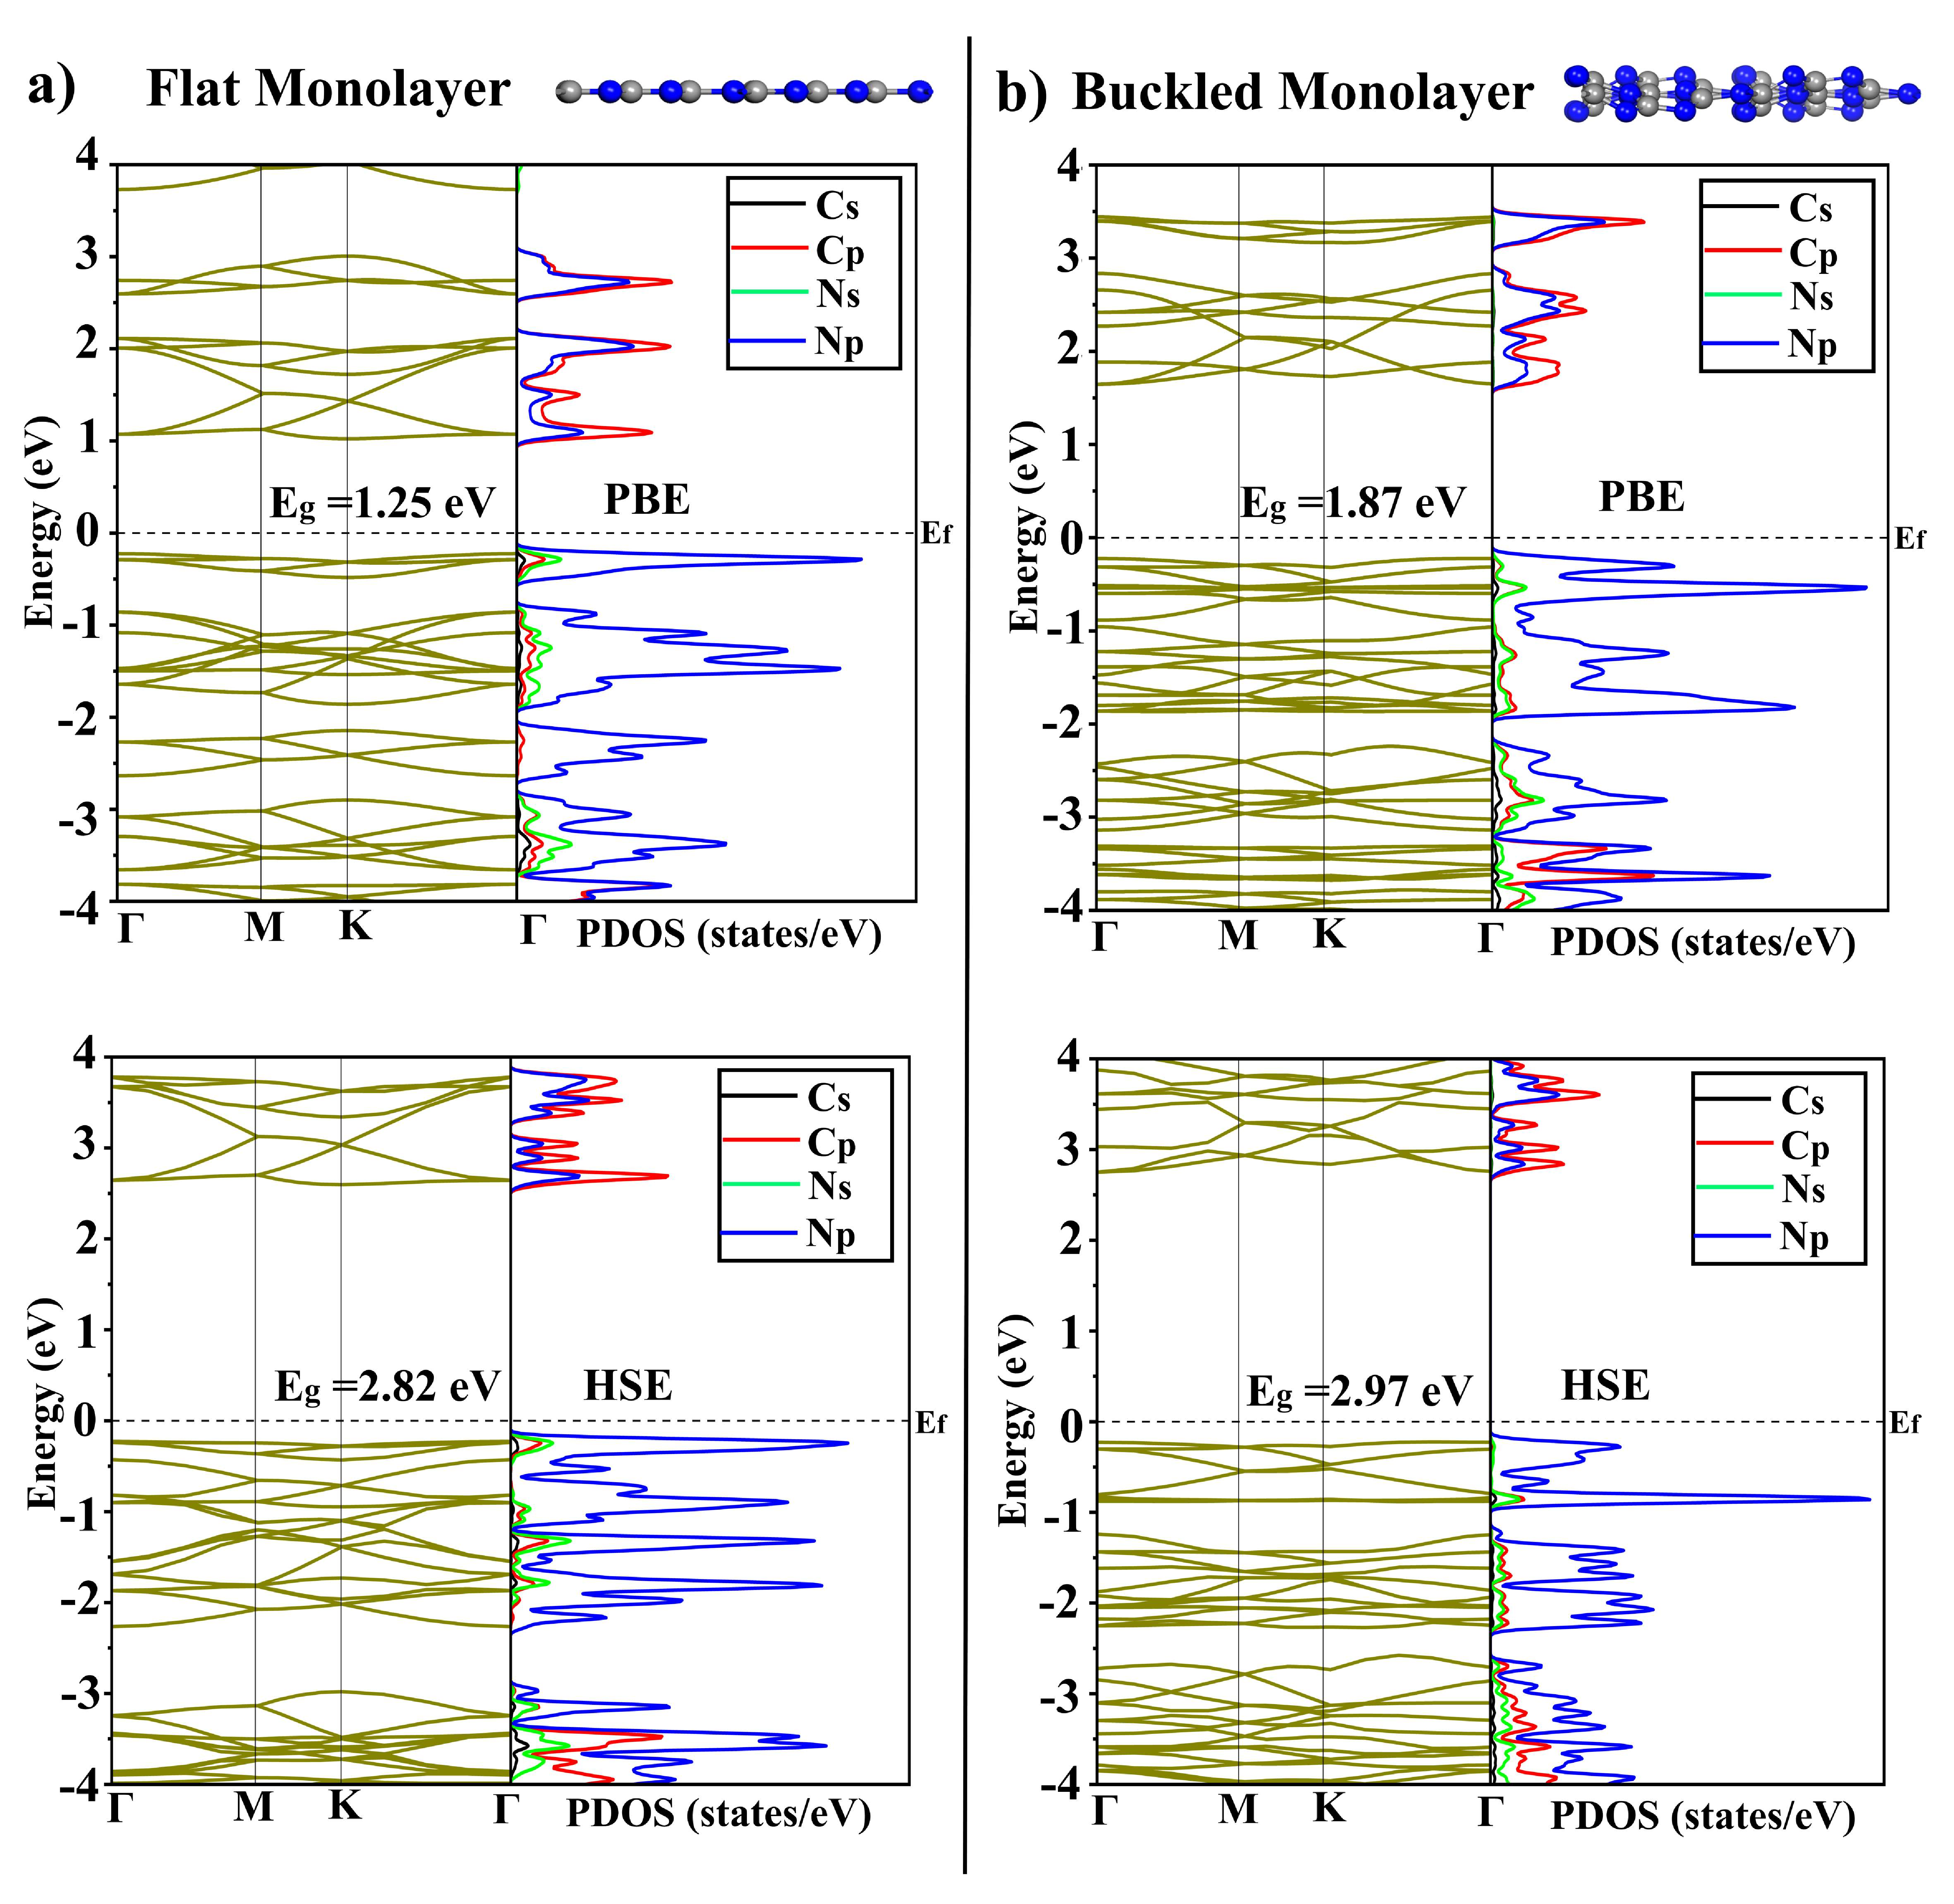
\includegraphics[width=6.0in]{Figures/Fig4.pdf}
 \caption{Electronic band structures and partial density of states (PDOS) of the planar and buckled heptazine-based g-C$_3$N$_4$ monolayers. 
 Upper panels PBE, lower panels HSE06.
 The Fermi level indicated by the dotted line is set to zero.} 
  \label{fig:Fig4} 
\end{figure*}


Fig.\ \ref{fig:Fig4} also shows the corresponding PDOS of both planar and buckled configurations, revealing the contributions of each atomic orbital type to the electronic band. In the valence band (VB), the major contribution originates mainly from the N-2p lone-pair orbital, while the conduction band (CB) is composed of the hybridization of C-2p and N-2p states. Moreover, both the band structure and PDOS of the buckled monolayer reveal an upward shift of the conduction-band edge compared to the planar model, resulting in a larger band gap (although we note that the Fermi energy is not defined meaningfully
in calculations of this type). 
Our observations are in good agreement with previous reports.\cite{Mortazavi2025AMonolayers,He2017EnhancementComposites,Zhu2018First-principleReview}

We now shift our attention to examining how different stacking motifs of the heptazine units influence the electronic properties of bulk g-C$_3$N$_4$. 
The layered structure of 3D-g-C$_3$N$_4$ introduces additional band dispersion along the out-of-plane direction, resulting in a narrower band gap compared to the isolated monolayer. For example, comparing the band structure plots in Figs.\ \ref{fig:Fig4} and \ref{fig:Fig5}, all the bulk stacking configurations exhibit smaller band gaps than the monolayer. For the flat models (at the PBE level), the band gap decreases from 1.25 eV in the monolayer to 0.59 eV (AA$_f$) and 1.03 eV (AB*$_f$), and from 2.82 eV to 1.93 eV (AA$_f$) and 2.06 eV (AB*$_f$) at the HSE06 level. A similar trend is also observed for buckled models, where the corresponding band gaps reduce from 1.87 eV in the monolayer to 1.59 eV (AA$_c$) and 1.60 eV (AB*$_c$) at the PBE level, and from 2.97 eV to 2.66 eV (AA$_c$) and 2.65 eV (AB*$_c$) using the HSE06 hybrid functional. 

\begin{figure*}
  \centering
  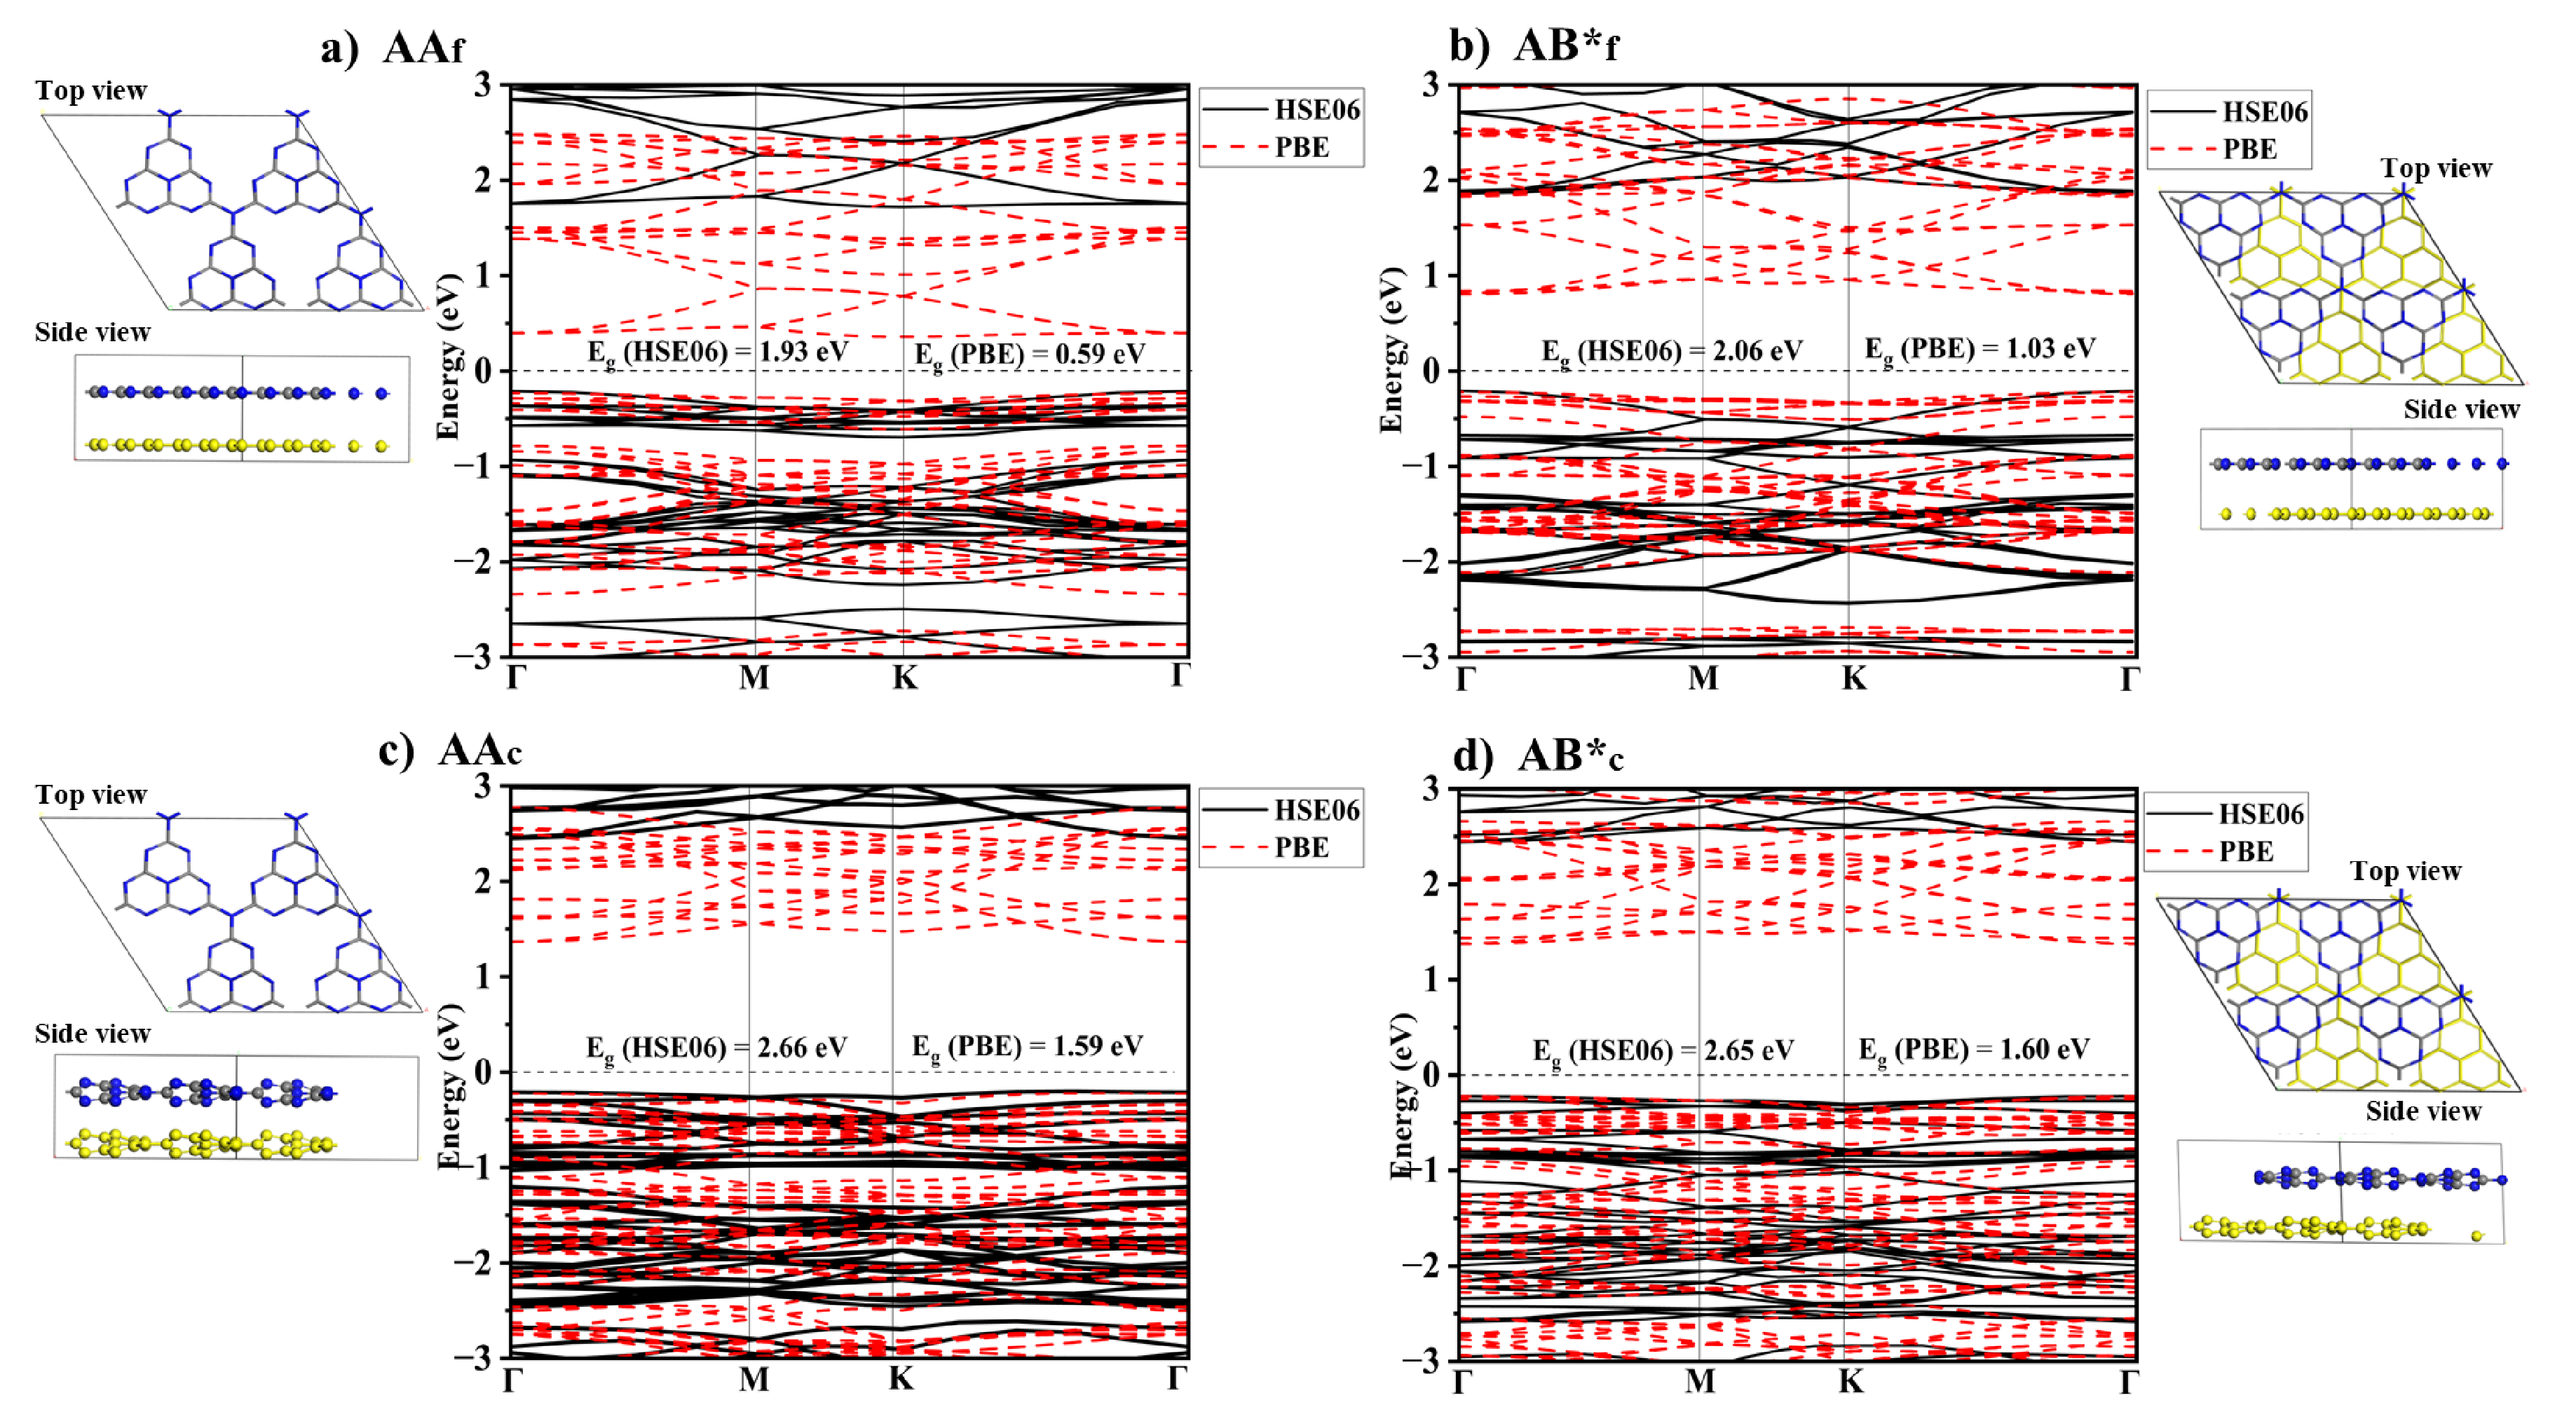
\includegraphics[width=6.5in]{Figures/Fig5.pdf}
 \caption{Electronic band structures of selected planar and buckled heptazine-based bulk g-C$_3$N$_4$ using two different XC functionals.
 The structures are illustrated to the sides.} 
  \label{fig:Fig5} 
\end{figure*}

Next, we extend our analysis to compare how different stacking arrangements (in the flat and corrugated models) influence the electronic response of bulk g-C$_3$N$_4$. It can be seen from Figs.\ \ref{fig:Fig5} and S1 that introducing a 180$^\circ$ rotation in the AA stacking registry, together with the presence of buckling in either stacking configuration, modulates the bulk electronic properties. While rotating the flat AA stacking motif moderately widens the band gap from 1.93 eV to 2.06 eV (HSE06), the introduction of buckling in the AA stacking (denoted as AA$_c$), even without rotation, results in a wider band gap of 2.66 eV (HSE06), which is in close agreement with experimental observations (2.7 eV).\cite{Chen2024SynthesisApplications} Moreover, applying a 180$^\circ$ rotation to the buckled AA stacking (AB*$_c$) induces minimal changes in the band gap, indicating that structural buckling exerts a more dominant role in determining interlayer electronic coupling compared with rotational misalignment alone. These findings suggest that 
lateral translation or combined rotation-translation of the layers,
for example by applying shear stress to the material,
could serve as a viable strategy to tune the bulk electronic properties of van der Waals layered g-C$_3$N$_4$. As shown in Fig. S2, the electronic response of the different corrugated stackings modulates the band dispersion and PDOS of bulk g-C$_3$N$_4$.

\begin{figure*}
  \centering
  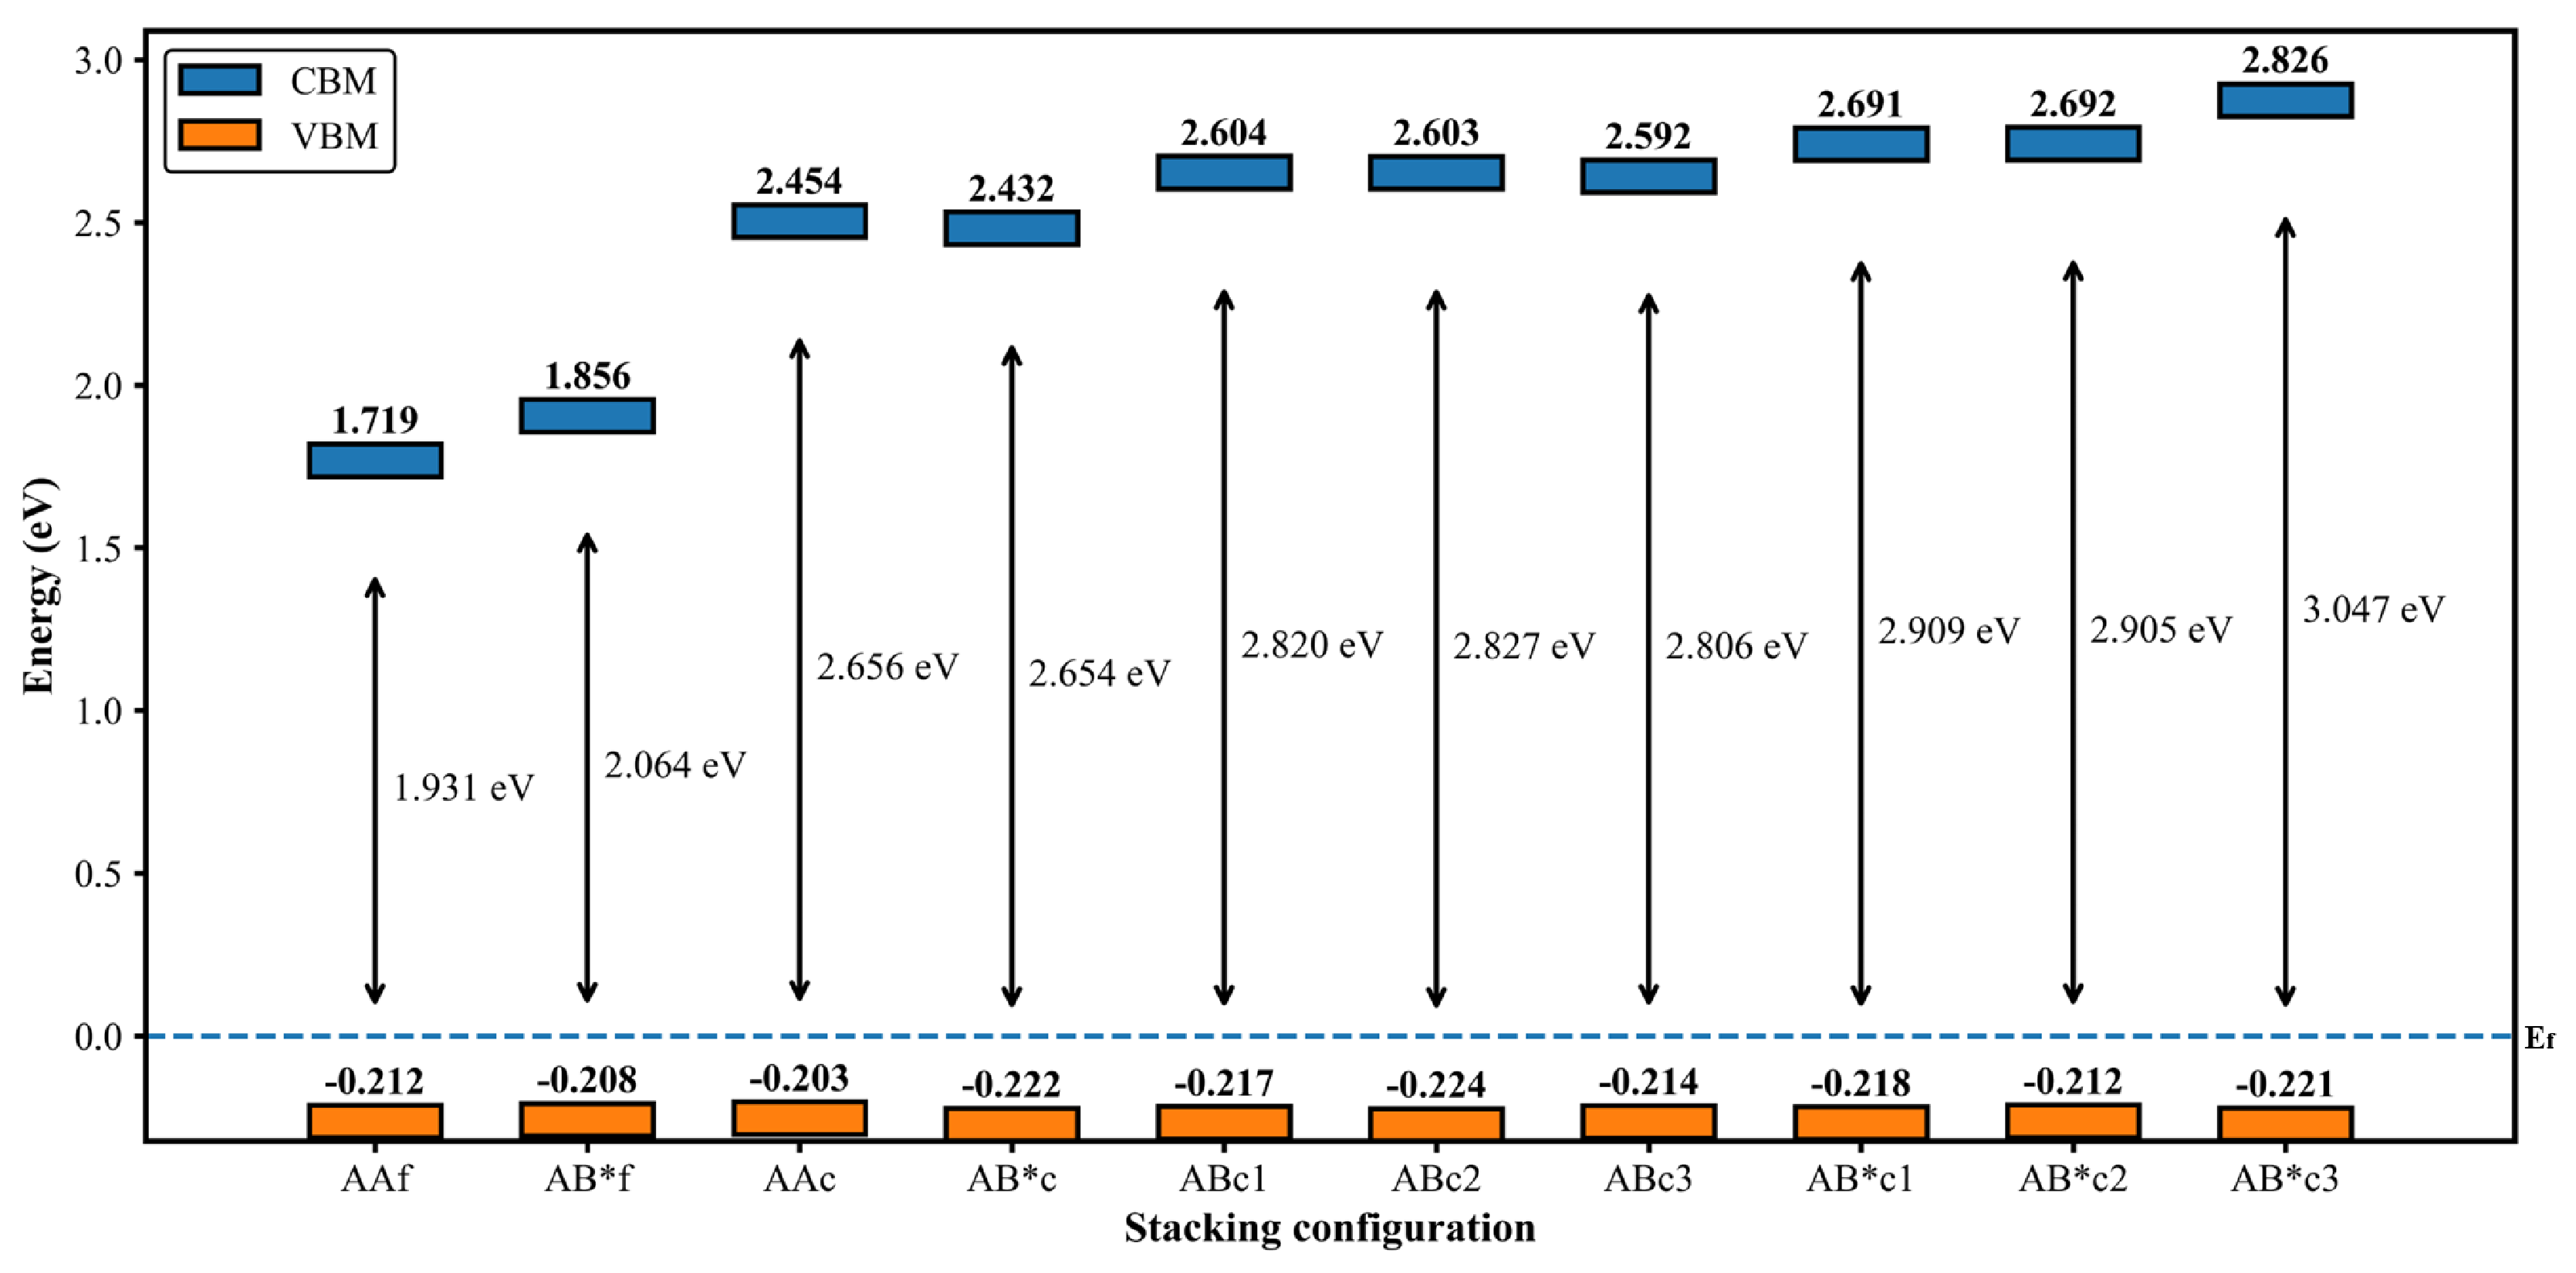
\includegraphics[width=6.2in]{Figures/Fig6.pdf}
 \caption{Relative band-edge positions and band gap variation (@HSE06 level) across different stacking configurations of heptazine-based g-C$_3$N$_4$. The Fermi level, E$_f$, assumed by Vasp is set to zero. The asterisk (*) and subscripts 'f' and 'c' refer to 180$^\circ$ rotation, flat and corrugated models, respectively.} 
  \label{fig:Fig6} 
\end{figure*}

A more detailed comparative analysis of the band gaps in Fig.\ \ref{fig:Fig6} quantifies the effect of these corrugated stacking variants. Relative to the unshifted corrugated models (i.e.\ AA$_c$, AB*$_c$), lateral translation increases the band gap by about 6\%. In contrast, the combined rotation–translation raises it by roughly 15\%, with the most stable structure, AB*$_{3c}$, exhibiting the widest band gap (3.05 eV) in these stacking series. Our findings reveal that while stacking of flat layers reduces the band gap, corrugation of stacked layers both enhances the thermodynamic stability and yields larger band gaps, consistent with the postulation of Im et al. \cite{Im2023StructureSimulations}. Accordingly, the band gap modulation approach demonstrated in this work may be extended to other two-dimensional materials to control their electronic properties, possibly including charge transport and photoresponse characteristics.

\subsection{Dopant roles in monolayer and bulk g-C$_3$N$_4$}
To investigate the influence of dopant on the 2D planar and 2D/3D buckled structural motifs of g-C$_3$N$_4$---and more importantly, how this is affected by the variations in structure discussed above---we select a representative non-metal dopant (P) and a metal dopant (Ni). Starting with the 2D buckled monolayer, we examined all possible substitutional P sites at C1-C6 and N1-N7 (Fig.\ \ref{fig:Fig2}), as well as the Ni interstitial site, using the defect formation energy expressions defined in Eqs.\ \ref{eq:formation_energy_sub} and \ref{eq:formation_energy_int}. Our calculations reveal that among the C dopant sites, P@C6 is the most thermodynamically favourable configuration, with a formation energy of 0.19 eV (see Figs. \ref{fig:Fig7} and S5). The P@N sites require significantly higher energies (0.60–1.90 eV, Fig. S6). 

 \begin{figure*}
  \centering
  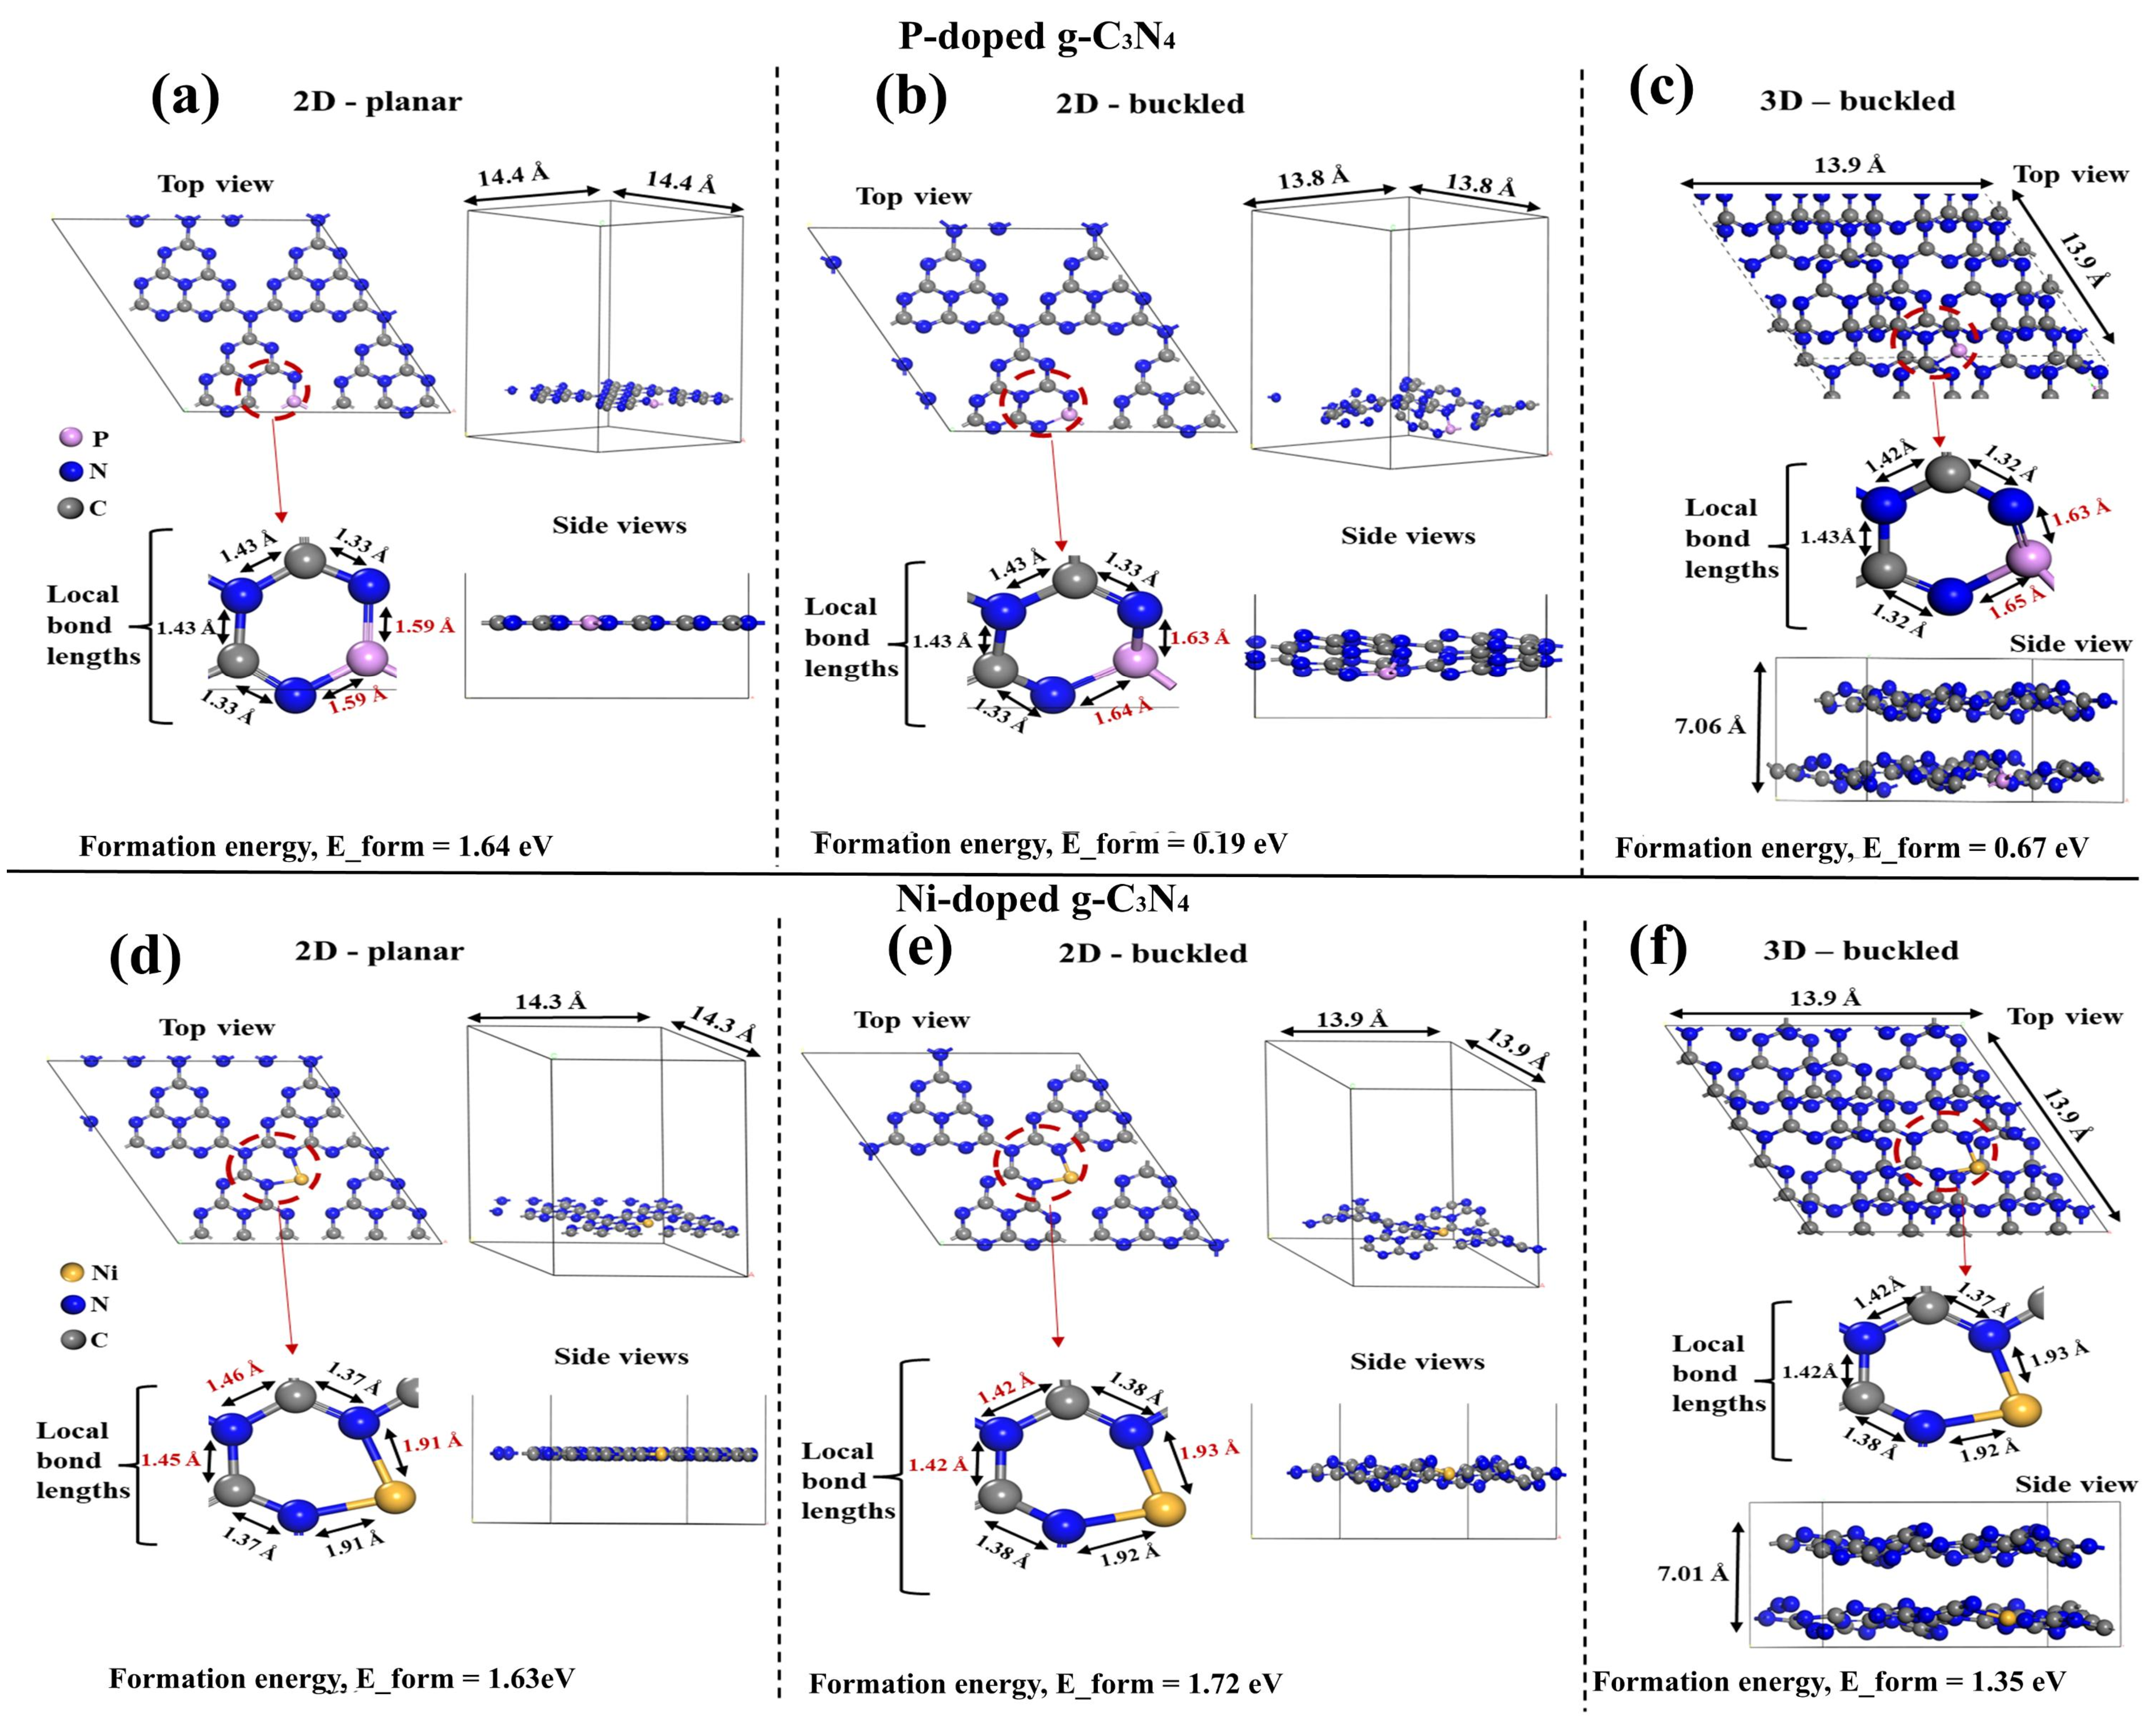
\includegraphics[width=6.6in]{Figures/Fig7.pdf}
 \caption{Structural configurations and formation energies of P and Ni dopants in planar and corrugated monolayer (2D) and bulk (3D) g-C$_3$N$_4$.} 
  \label{fig:Fig7} 
\end{figure*}

The P@C6 site was used as a model defect to examine how dopant accommodation varies with buckling and stacking structure, comparing the 2D-planar and buckled monolayers with the buckled 3D-stacked g-C$_3$N$_4$. Fig. \ref{fig:Fig7} shows that the formation energy changes dramatically from the planar sheet (1.64 eV) to the buckled monolayer (0.19 eV), whereas the 3D-buckled structure exhibits an intermediate stability (0.67 eV). The variation in formation energies, despite using the same dopant sites (P@C6) across all structures, indicates that each host lattice accommodates the dopant differently. In the planar monolayer (Fig.\ \ref{fig:Fig7}a), the P dopant is constrained by the in-plane symmetry of the lattice, resulting in a P-N bond length of 1.59~\text{\AA}, longer than the intrinsic C-N bond length of 1.33~\text{\AA}, giving rise to local strain. In contrast, the buckled monolayer alleviates this strain by allowing the dopant to relax out of plane, as reflected by the P–N bond length (1.63–1.64 ~\text{\AA}, Fig.\ \ref{fig:Fig7}b). 
In the 3D-buckled structure (Fig.\ \ref{fig:Fig7}c), the local bonding geometry around the P dopant is nearly identical to that of the buckled monolayer, with comparable P–N distances. However, the difference in the formation energies between the 2D buckled monolayer and the 3D buckled lattice can be attributed to the long-range interlayer interactions in the bulk and not from the local bonding environment. Similarly for the Ni dopant at the same interstitial sites across the planar, buckled monolayer, and 3D-buckled structures (Fig.\ \ref{fig:Fig7}d-f), the formation energies vary with 1.63 eV for planar 2D, 1.72 eV for buckled 2D, and 1.35 eV for buckled 3D.  The variation in dopant energetics between P and Ni at identical sites across flat, buckled, and layered g-C$_3$N$_4$ structures demonstrates that accurate theoretical modelling of g-C$_3$N$_4$ must account for intrinsic structural stability as well as the influence of interlayer coupling. 

\begin{figure*}
  \centering
  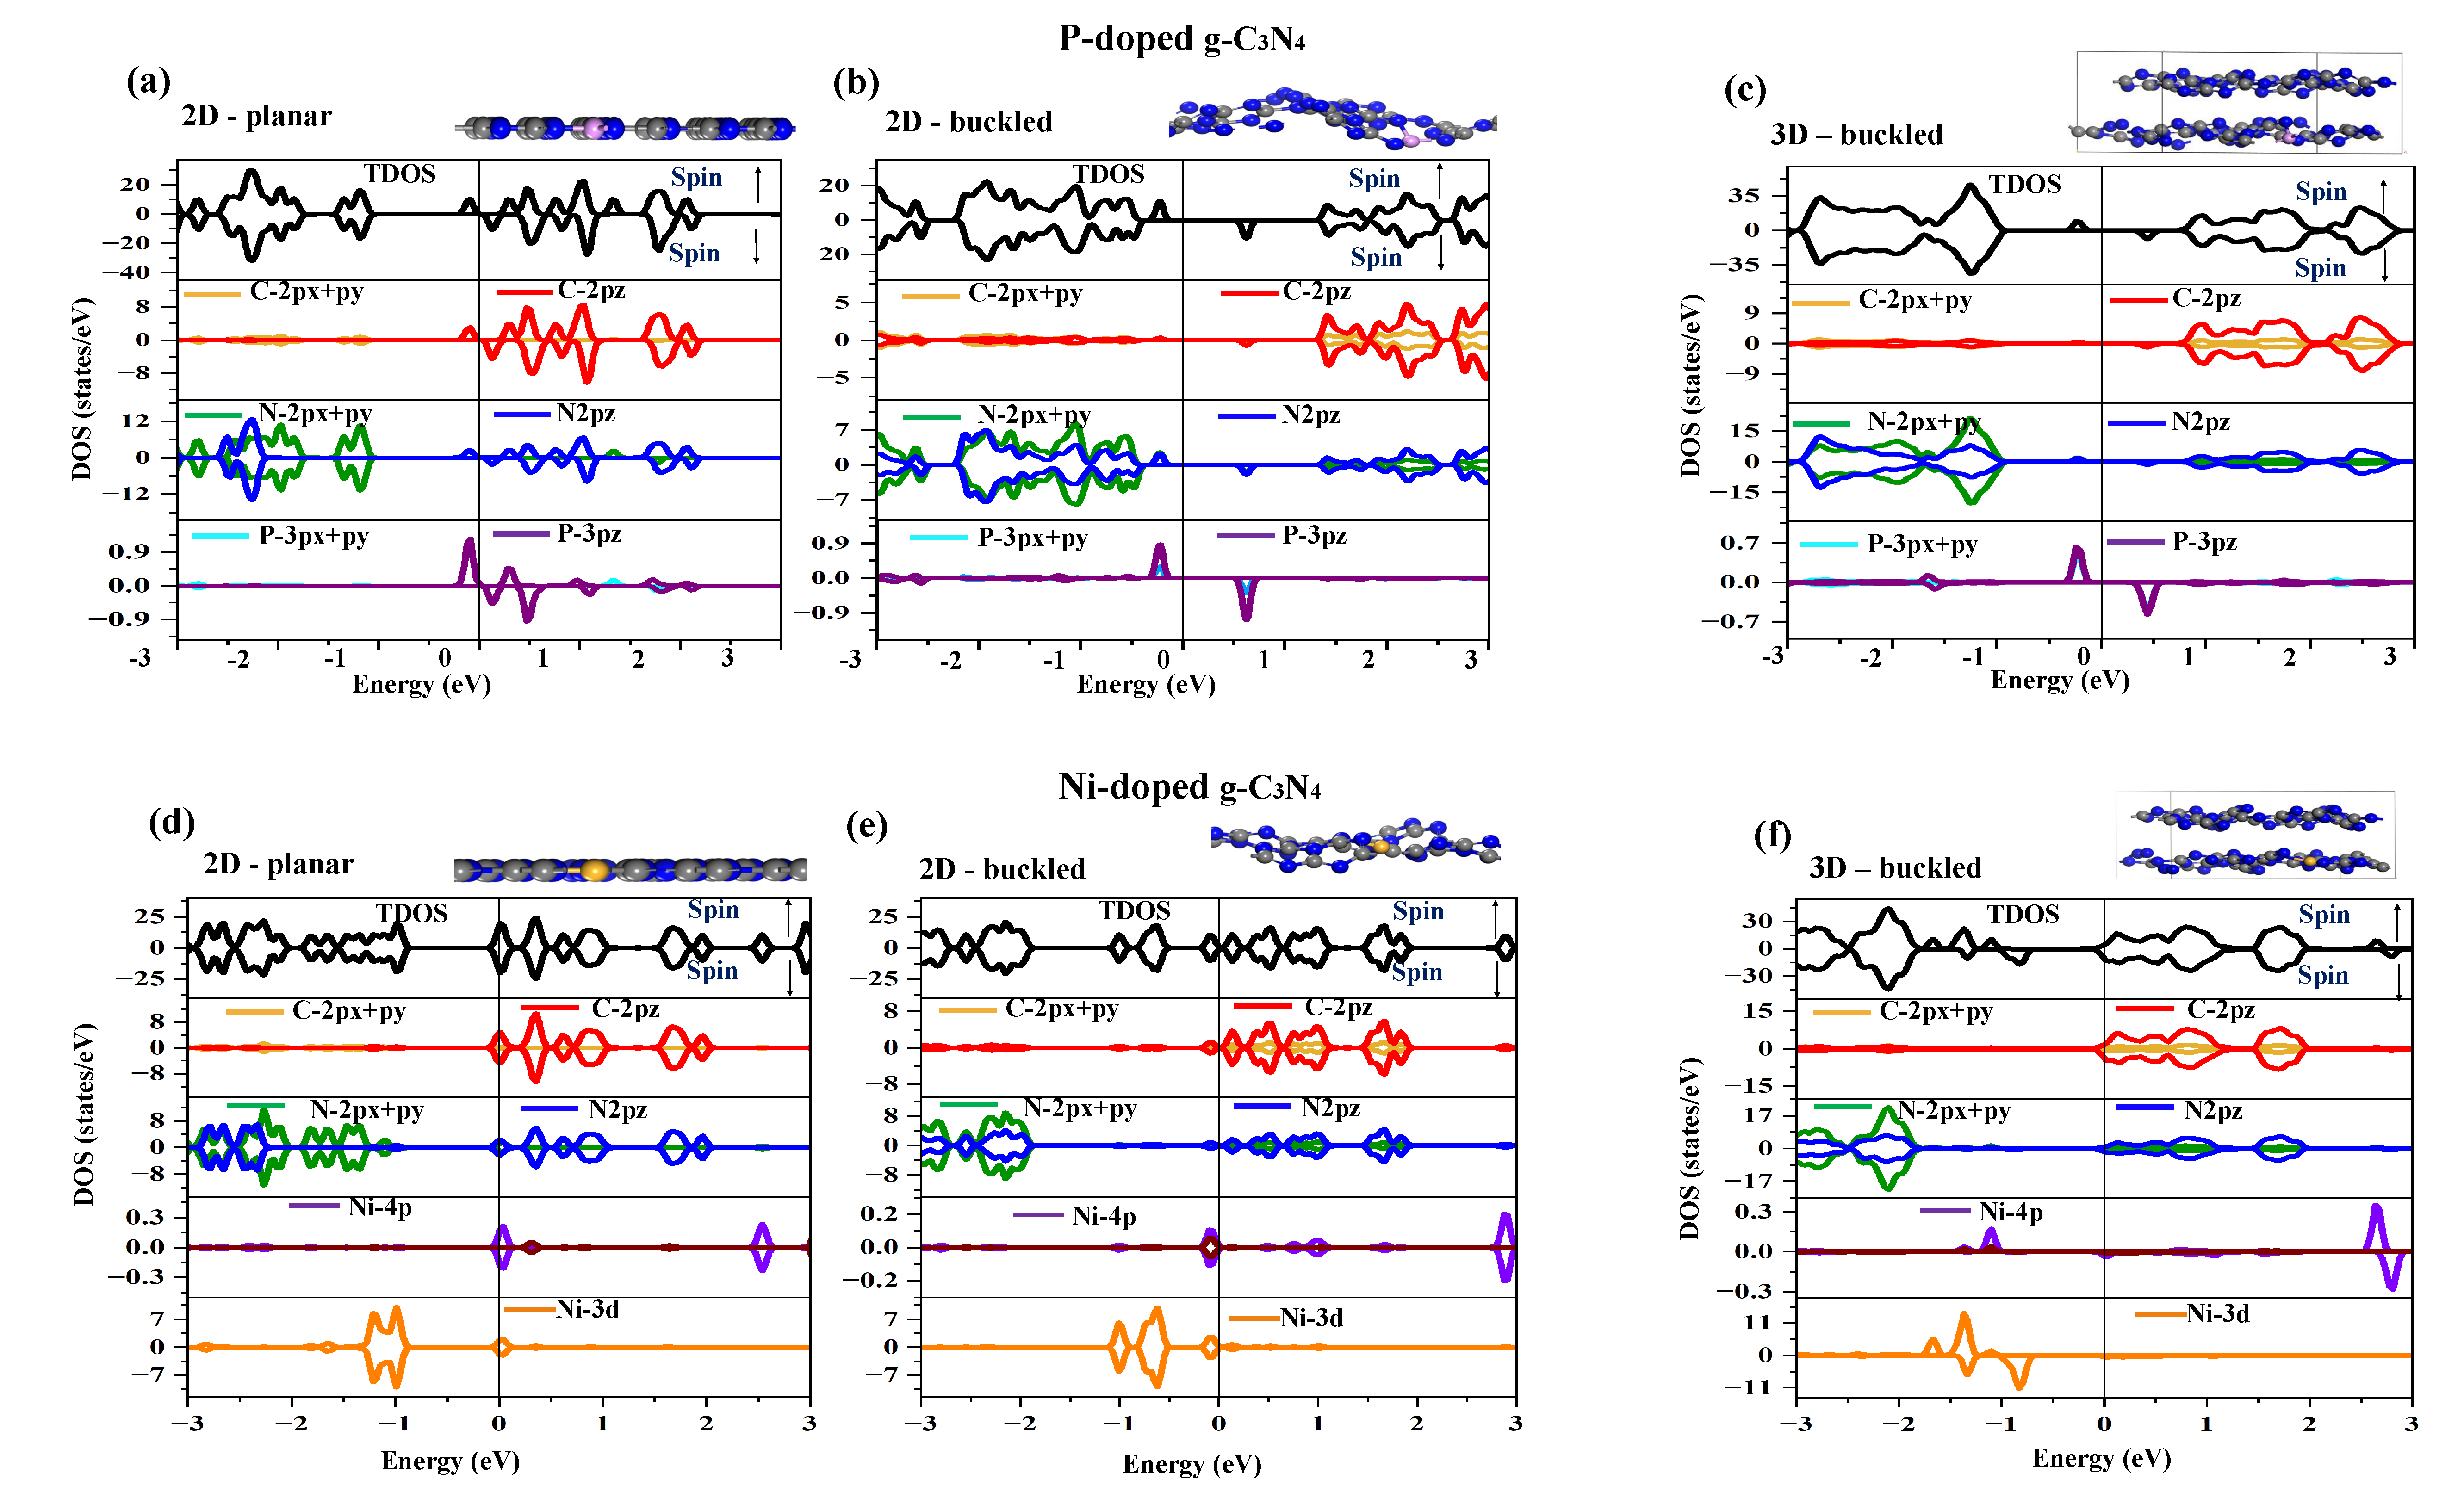
\includegraphics[width=7.0in]{Figures/Fig8.pdf}
 \caption{Spin-polarized projected density of states (PDOS) of P- and Ni-doped g-C$_3$N$_4$ in planar 2D, buckled 2D, and buckled 3D configurations.} 
  \label{fig:Fig8} 
\end{figure*}

The buckling and stacking structure influenced the effect of dopants on the calculated electronic structure.
Figs. \ref{fig:Fig8}a--c and S8a--c show that doping with P does not significantly alter the bulk band structure of the underlying g-C$_3$N$_4$ structure.  
The significant change to the electronic structure is the introduction of mid-gap states associated with the P dopant atom.  For the neutral systems modelled here, a single electron occupies one of these states, with the opposite spin state remaining unoccupied.  Clearly, such mid-gap states could be expected to have a significant effect on the photocatalytic properties of doped g-C$_3$N$_4$.

The position of these states within the gap, and the separation between the occupied and unoccupied states, are strongly affected by the modelled structure.  The planar 2D structure yields a small separation between the occupied and unoccupied states, with both lying close to the conduction band of g-C$_3$N$_4$.  Allowing the monolayer to buckle out of the plane separates the occupied and unoccupied states by around 1~eV, with the occupied state lying close to the valance band.  Stacking g-C$_3$N$_4$ into a bulk structure causes both mid gap states to move higher in the band gap.

\begin{figure*}
  \centering
  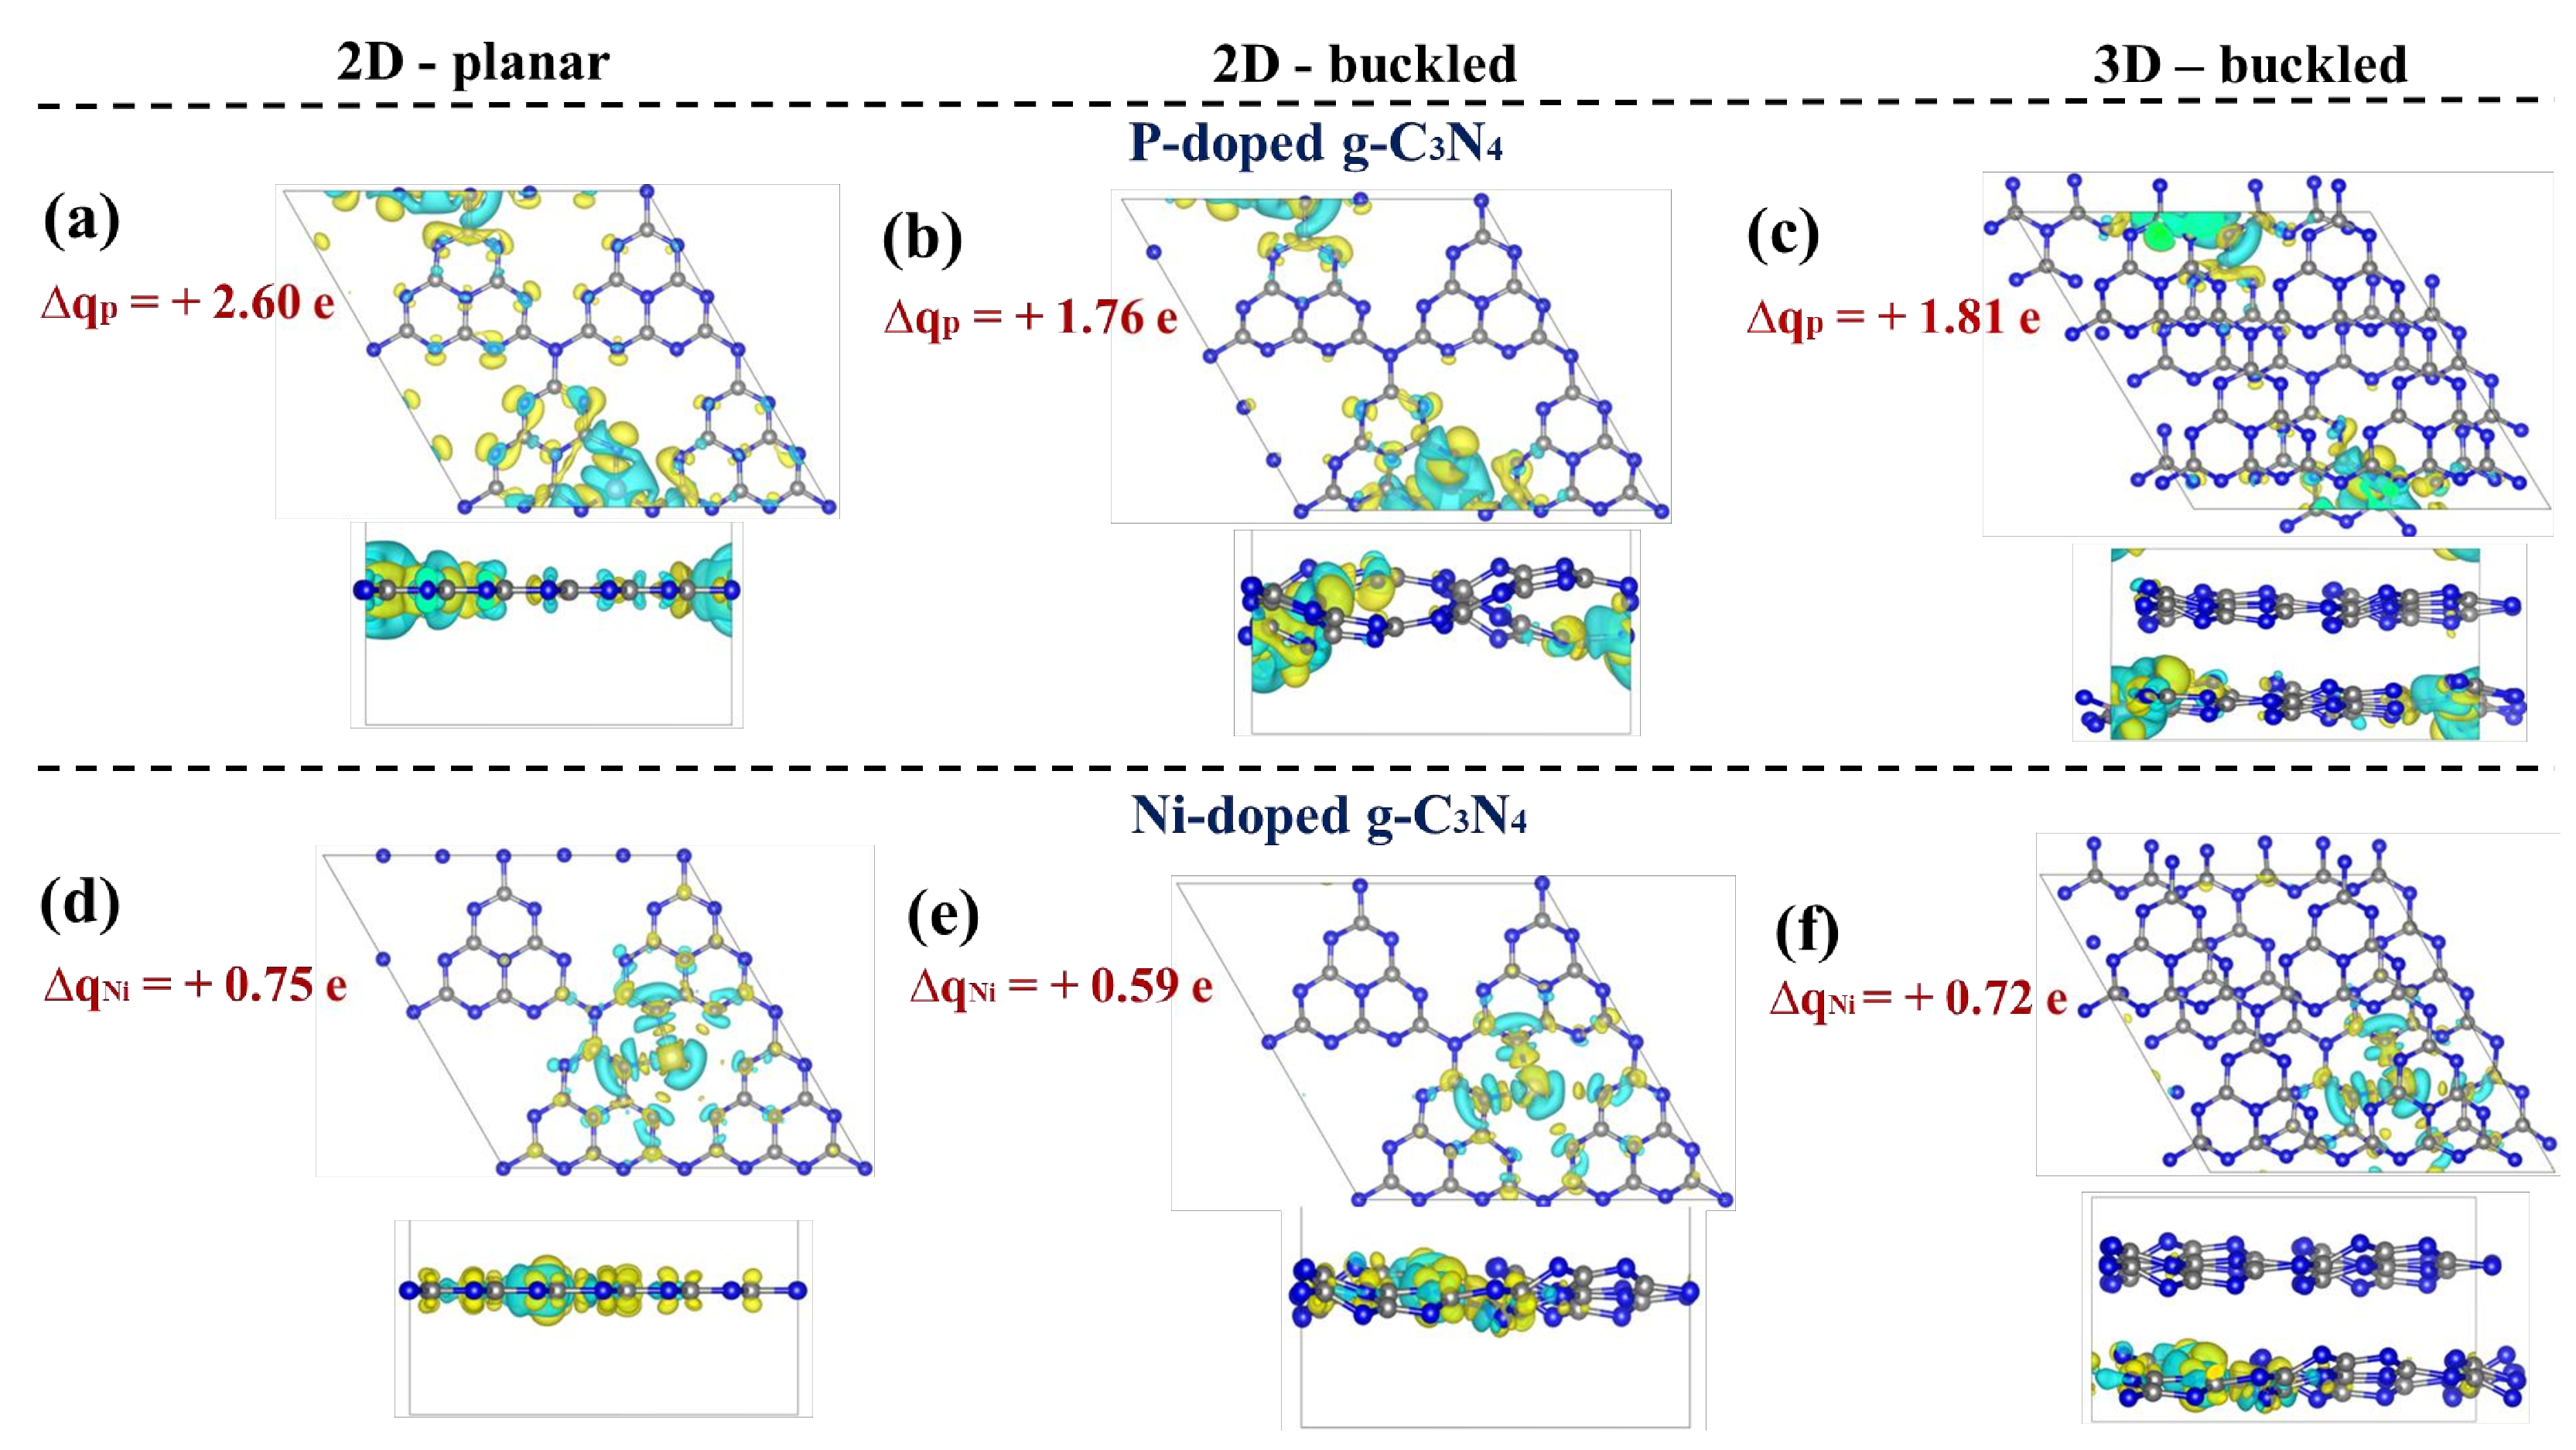
\includegraphics[width=6.5in]{Figures/Fig9.pdf}
 \caption{Charge density difference (CDD) distributions and Bader charge variations ($\Delta$q) of P- and Ni-doped g-C$_3$N$_4$ in planar 2D, buckled 2D, and buckled 3D structures. The yellow and cyan regions denote electron accumulation and depletion, respectively. The isosurface is taken as 0.003 e/bohr$^3$.} 
  \label{fig:Fig9} 
\end{figure*}

Charge density difference (CDD) and Bader charge transfer 
calculations for these P-doped structures are represented in Fig.\ \ref{fig:Fig9}a--c.  These again demonstrate significant differences between the different
g-C$_3$N$_4$ parent structures, with significant differences between the amount of charge transferred to the g-C$_3$N$_4$ structure depending on whether the doped parent is planar, buckled, or in bulk.

For g-C$_3$N$_4$ doped with interstitial Ni, the parent band structure was again largely unchanged from the undoped material's band structure for the monolayer cases (Figs.\ \ref{fig:Fig8}d,e and S8d,e).  Occupied Ni 4p states were introduced at the top of the gap for the flat structure, with Ni 3d lying at the bottom of the gap.  The wider gap of the more stable buckled monolayer again presented occupied Ni 4p states at the top of the gap, but exposed Ni 3d states lying in the parent material band gap at slightly destabilized energies.  Introducing a Ni dopant to the bulk AB$_{3c}$ structure (Figs.\ \ref{fig:Fig8}f and S8f) opened the parent material band gap to almost 2 eV, with occupied Ni 3d states again appearing in the lower half of the parent gap.  In this case, occupied Ni 4p states were stabalised to similar energies to the Ni 3d states, maintaining a nominal intrinsic band gap of around 0.7~eV.
Fig.\ \ref{fig:Fig9}d--f indicates that the electron transfer from the Ni dopant was similar in the planar 2D and buckled bulk cases but reduced by more than 20\% when the monolayer was allowed to buckle to a more stable configuration.

\subsection{Experimental verification}
To this point, this paper, along with others, presents a clear case based on 
DFT that the ``graphitic'' layers of g-C$_3$N$_4$ are not in fact flat planes like graphite, but rather strongly buckled structures.  Although modern DFT approaches are reliable, sceptics may question whether this behaviour is an artefact of the sophistication of the exchange-correlation functional, the treatment of dispersion, or other deficiencies of the theory.

\begin{figure}
  \centering
  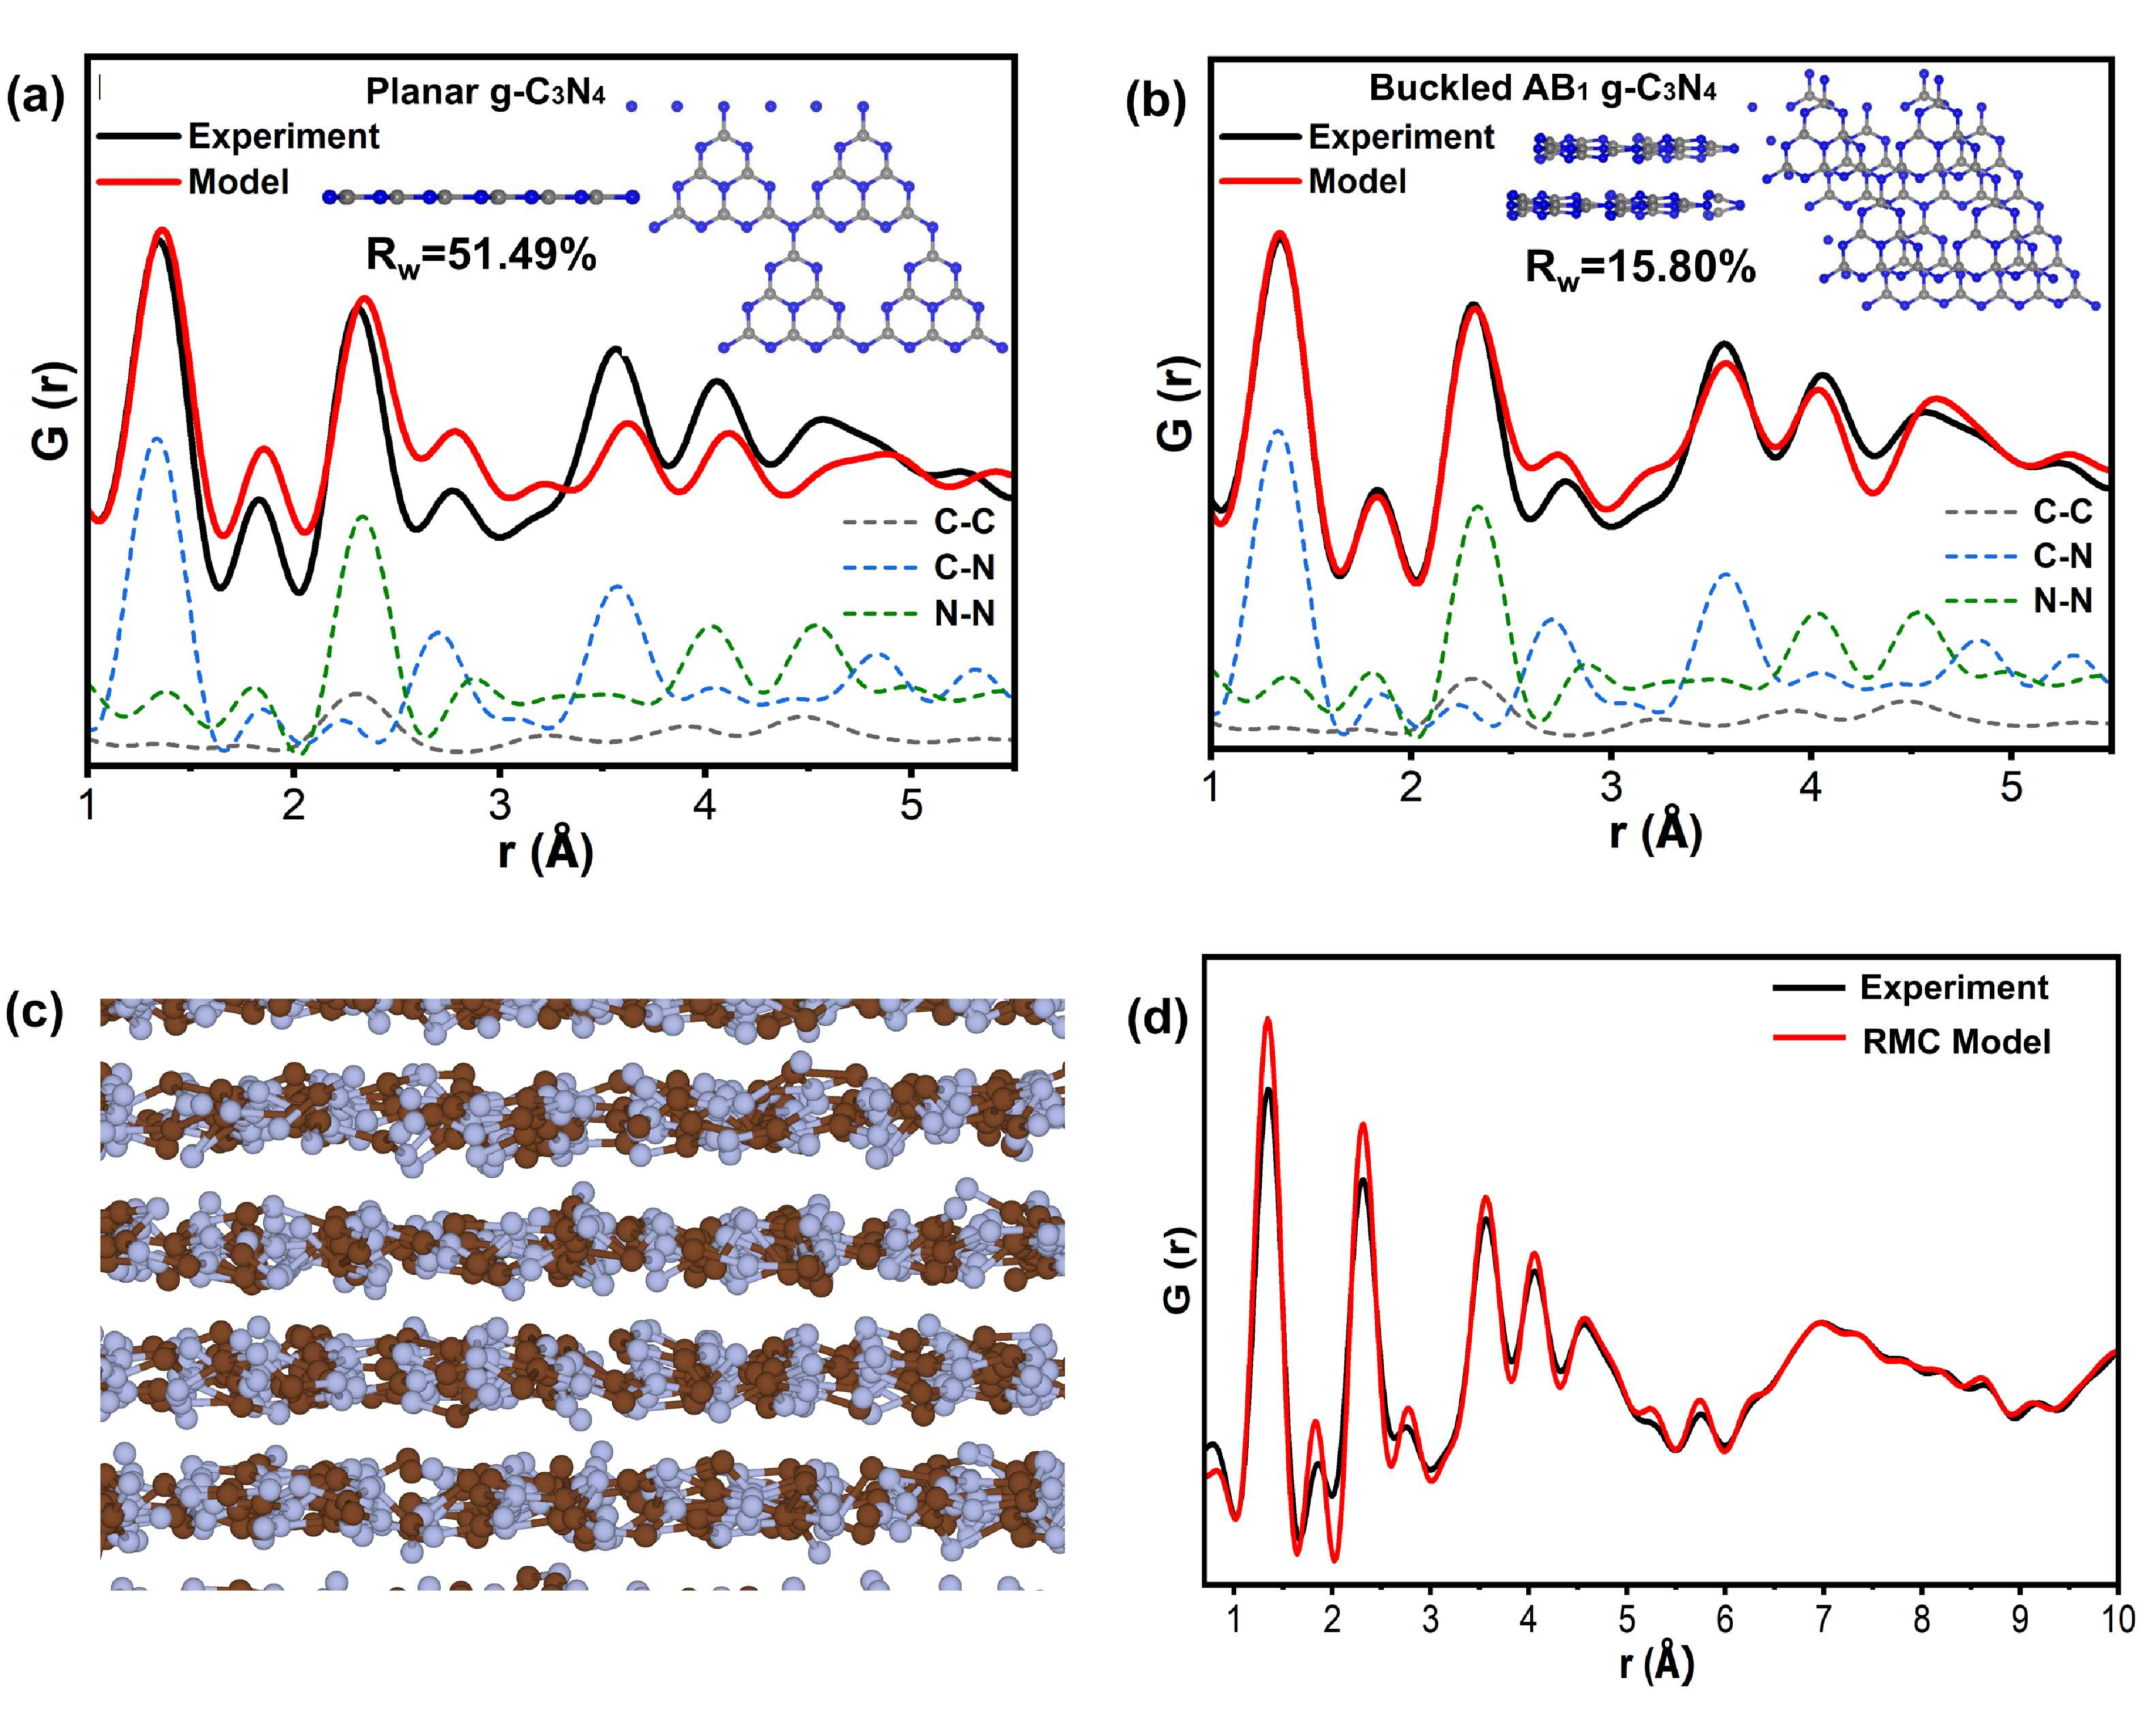
\includegraphics[width=3.5in]{Figures/Fig10.pdf}
 \caption{%
(a,b) Experimental X-ray total scattering $G(r)$ (black) compared with planar and buckled AB-stacked g-C$_3$N$_4$ models (red), showing poor agreement for the planar structure ($R_\mathrm{w}=51.49\%$) and markedly improved agreement for the buckled AB model ($R_\mathrm{w}=15.80\%$); dashed curves denote C--C, C--N, and N--N partial correlations.
(c) Ball-and-stick representation of the RMC-refined g-C$_3$N$_4$ structure fitted to X-ray total scattering data, showing part of the 10\,000-atom supercell viewed along $[11\bar{2}0]$.
(d) Comparison of the experimental $G(r)$ (black) with the final RMC model (red).%
}
  \label{fig:Fig10} 
\end{figure}

As a final independent piece of evidence that the layers of g-C$_3$N$_4$ are indeed buckled away from planarity, we present some experimental evidence.  X-ray total scattering data for g-C$_3$N$_4$ was simulated via reverse Monte Carlo calculation with the RMCProfile code.\cite{Tucker2007RMCProfile:Materials, Liu2025HarnessingCapacitors}
During the RMC run, the atoms of g-C$_3$N$_4$ moved consistently away from planar structures in order to give a good fit to the X-ray scattering data, which could not be obtained from a structure comprised of flat planes of atoms.  A side view of this real-space structure is shown in Fig.\ \ref{fig:Fig10}.  

The out-of-plane displacements generated by the RMC simulation are similar in magnitude to those exhibited by our DFT structures.  Note that the RMC structures maintained atomic positions consistent with the structure as a heptazine polymer throughout.
Further details of these and related RMC simulations will be presented in a related paper. \cite{Adnan2026atomicallycoordinatednonmetal}





\section{Conclusions}
In this study, we systematically explore the structural stability of heptazine-based g-C$_3$N$_4$ from a monolayer to different stacking configurations and how the presence of dopants in these configurations modulates the structural and electronic properties.
Our results show that: 
\begin{itemize}
    \item 
    The widely assumed planar ($P\bar{6}m2$) model of g-C$_3$N$_4$ is neither energetically stable nor a reasonable approximation to the structure of ordered g-C$_3$N$_4$. Allowing out-of-plane atomic relaxation yields a lower-energy buckled structure that alleviates the in-plane N-lone-pair repulsion inherent to the planar model, whereas doping with heteroatoms is not required to induce buckling.
    \item 
    In the layered heptazine-based g-C$_3$N$_4$ structure, the stacking patterns previously demonstrated to be the lowest in energy for flat layers are significantly higher in energy than other stacking patterns when the layers are buckled.
    \item 
    The electronic structure of g-C$_3$N$_4$ is sensitive to both buckling and stacking registry. Although buckling generally widens the band gap relative to the planar monolayer, different corrugated stacking configurations yield distinct band gap values, which could potentially be an effective mechanism for tuning the electronic properties of bulk g-C$_3$N$_4$. For example, the corrugated stackings ($P1$ symmetry) uncovered in this study display varied electronic responses, with the band gaps of certain stacking configurations aligning closely with experimentally reported values. The most stable structure found in this work was the one labelled $AB^*_{3c}$ while $AB_{3c}$ showed the best match to the experimental band gap (calculated at the HSE06 level).
    \item 
    The calculated stability and electronic effect of representative metal and non-metal single atom dopants is strongly impacted by the treatment of both buckling and stacking.
\end{itemize}

We present a number of corrugation patterns that were calculated to be 
lower in energy than any of those previously reported.  Key to these
lower energy structures was the use of a $2 \times 2$ supercell 
within each plane, allowing adjacent heptazine units to buckle in opposite directions.  The hexagonal structure of g-C$_3$N$_4$ suggests this 
alternation of structure may be frustrated in the third equivalent in-plane direction.

Within these corrugated structures, P and Ni dopants exhibit markedly different electronic responses compared with the flat model, demonstrating that dopant functionality depends primarily on the host structural motif. As such, reliable property prediction and rational design of both pristine and doped g-C$_3$N$_4$ require careful consideration of accurate structural models to enable the development of high-performance g-C$_3$N$_4$ photocatalysts.
In particular, studying the effect of dopants by using DFT calculations based on either flat or buckled g-C$_3$N$_4$ monolayers is likely to be misleading if the target material is a synthesisable (i.e.\ multilayer or bulk) doped g-C$_3$N$_4$.  Such calculations yield incorrect predictions of both the propensity of dopants to enter the g-C$_3$N$_4$ lattice and the effects of such dopants on the electronic (and hence photocatalytic) properties of  the doped material.








\section*{Conflicts of interest}
There are no conflicts of interest to declare.

\section*{Data availability}
The data supporting the findings of this study have been included in this article and in the supplementary information (SI). See DOI:00.0000/00000000.

\section*{Acknowledgement}
This work was supported by the Australian Research Council Centre of Excellence for Carbon Science and Innovation (CE230100032), the Australian Laureate Fellowship program (FL210100017), and the Linkage Project (LP200200472). 
This research was undertaken with the assistance of resources from the National Computational Infrastructure (NCI Australia), an NCRIS-enabled capability supported by the Australian Government.
Access to NCI resources was facilitated by the UNSW HPC Scheme (\url{https://doi.org/10.26190/PMN5-7J50}). 

%\clearpage 
\bibliographystyle{rsc}
\bibliography{references, references-2} 

\end{document}